\RequirePackage{etoolbox}
\csdef{input@path}{%
 {sty/}% cls, sty files
 {img/}% eps files
 {art/}% pdf figures
}%
\csgdef{bibdir}{bib/}% bst, bib files

\documentclass[ba]{imsart}
%
\pubyear{0000}
\volume{00}
\issue{0}
\doi{0000}
\firstpage{1}
\lastpage{1}


%
\usepackage{amsthm}
\usepackage{amsmath}
\usepackage{natbib}
\usepackage[colorlinks,citecolor=blue,urlcolor=blue,filecolor=blue,backref=page]{hyperref}
\usepackage{graphicx}

%\usepackage{palatino}
%\usepackage{parskip}


%\usepackage{setspace}
\usepackage{graphicx}
\usepackage{wrapfig}
\usepackage{epstopdf}
\usepackage{subcaption}
\usepackage{multirow}
\usepackage{nicefrac}

\usepackage{float}
\usepackage{titlesec}
\titleformat{\subsubsection}[runin]
  {\normalfont\large\bfseries}{\thesubsubsection}{1em}{}

%% Please use the following statements for
%% managing the text and math fonts for your papers:
%\usepackage{times}
%%\usepackage[cmbold]{mathtime}
%\usepackage{bm}

\usepackage{array}

% this order is important
%\RequirePackage[hyphens]{url}
%\RequirePackage[colorlinks,citecolor=blue,urlcolor=blue]{hyperref}
%\usepackage[authoryear]{natbib}
\usepackage[plain,noend]{algorithm2e}

\startlocaldefs
% ** Local definitions **
\newcolumntype{L}[1]{>{\raggedright\let\newline\\\arraybackslash\hspace{0pt}}m{#1}}
\newcolumntype{C}[1]{>{\centering\let\newline\\\arraybackslash\hspace{0pt}}m{#1}}
\newcolumntype{R}[1]{>{\raggedleft\let\newline\\\arraybackslash\hspace{0pt}}m{#1}}

 \newcommand{\beginsupplement}{%
        \setcounter{equation}{0}
				\setcounter{page}{0}
				\setcounter{table}{0}
				\setcounter{section}{0}
				\setcounter{figure}{0}

			\numberwithin{table}{section}
			\renewcommand{\theequation}{S.\arabic{equation}}
			\renewcommand{\thesection}{S.\arabic{section}}
			\renewcommand{\thesubsection}{S.\arabic{section}.\arabic{subsection}}
			\renewcommand{\thepage}{S.\arabic{page}}
			\renewcommand{\thetable}{S.\arabic{table}}
			\renewcommand{\thefigure}{S.\arabic{figure}}
}
% For compressing some space: 
%\setlength{\textfloatsep}{10pt plus 1.0pt minus 2.0pt}
%\setlength{\floatsep}{12.0pt plus 2.0pt minus 5.0pt}
%\setlength{\intextsep}{12.0pt plus 2.0pt minus 5.0pt}
%\setlength{\belowcaptionskip}{-2pt}
%
%\setlength{\textheight}{9in}
%\setlength{\textwidth}{6in}
%\setlength{\topmargin}{-36pt}
%\setlength{\oddsidemargin}{0pt}
%\setlength{\evensidemargin}{0pt}

%% Special shortcuts for us
\def\Polya{P{\'o}lya}
\def\CS{Cauchy-Schl\"omilch}
\def\PG{P{\'o}lya-Gamma}
\def\sql{$\sqrt{\text{Lasso}}$}
\def\sqdl{Dirichlet-$\sqrt{\text{Lasso}}$}

\usepackage{array}
\graphicspath{{./art/}}

%
% Math commands by Thomas Minka 
%
% Revised by Jyotishka Datta & Brandon Willard
% Acknowledgement: JD received this from Prof. Alan Qi.
%


%% Special shortcuts for us
\def\Polya{P{\'o}lya}
\def\CS{Cauchy-Schl\"omilch}
\def\PG{P{\'o}lya-Gamma}

%\setlength{\textfloatsep}{10pt plus 1.0pt minus 2.0pt}
%\setlength{\floatsep}{12.0pt plus 2.0pt minus 5.0pt}
%\setlength{\intextsep}{12.0pt plus 2.0pt minus 5.0pt}
%\setlength{\belowcaptionskip}{-2pt}

%\def\distrib{\mathrel{\ooalign{%
%  \raisebox{0.75\height}{{\small{ind}}}\cr\hidewidth$\sim$\hidewidth\cr}}}
%  
\newcommand{\var}{{\rm var}}
\newcommand{\Tr}{^{\rm T}}
\newcommand{\rmlog}{\rm log}
\newcommand{\vtrans}[2]{{#1}^{(#2)}}
\newcommand{\kron}{\otimes}
\newcommand{\schur}[2]{({#1} | {#2})}
\newcommand{\schurdet}[2]{\left| ({#1} | {#2}) \right|}
\newcommand{\had}{\circ}
\newcommand{\diag}{{\rm diag}}
\newcommand{\invdiag}{\diag^{-1}}
\newcommand{\rank}{{\rm rank}}
% careful: ``null'' is already a latex command
\newcommand{\nullsp}{{\rm null}}
\newcommand{\tr}{{\rm tr}}
\renewcommand{\vec}{{\rm vec}}
\newcommand{\vech}{{\rm vech}}
\renewcommand{\det}[1]{\left| #1 \right|}
\newcommand{\pdet}[1]{\left| #1 \right|_{+}}
\newcommand{\pinv}[1]{#1^{+}}
\newcommand{\erf}{{\rm erf}}
\newcommand{\hypergeom}[2]{{}_{#1}F_{#2}}

% boldface characters
\renewcommand{\a}{{\bf a}}
\renewcommand{\b}{{\bf b}}
\renewcommand{\c}{{\bf c}}
\renewcommand{\d}{{\rm d}}  % for derivatives
\newcommand{\e}{{\rm e}} % for exponentials
\newcommand{\f}{{\bf f}}
\newcommand{\g}{{\bf g}}
\newcommand{\h}{{\bf h}}
%\newcommand{\k}{{\bf k}}
% in Latex2e this must be renewcommand
\renewcommand{\k}{{\bf k}}
\newcommand{\m}{{\bf m}}
\newcommand{\n}{{\bf n}}
%\renewcommand{\o}{{\bf o}}
\newcommand{\p}{{\bf p}}
%\newcommand{\q}{{\bf q}}
\renewcommand{\r}{{\bf r}}
\newcommand{\s}{{\bf s}}
\renewcommand{\t}{{\bf t}}
\renewcommand{\u}{{\bf u}}
\renewcommand{\v}{{\bf v}}
\newcommand{\w}{{\bf w}}
%\newcommand{\x}{{\bf x}}
\newcommand{\y}{{\bf y}}
%\newcommand{\z}{{\bf z}}
\newcommand{\A}{{\bf A}}
\newcommand{\B}{{\bf B}}
\newcommand{\C}{{\bf C}}
\newcommand{\D}{{\bf D}}
\newcommand{\E}{{\bf E}}
\newcommand{\F}{{\bf F}}
%\newcommand{\G}{{\bf G}}
\renewcommand{\H}{{\bf H}}
\newcommand{\I}{{\bf I}}
\newcommand{\J}{{\bf J}}
\newcommand{\K}{{\bf K}}
\renewcommand{\L}{{\bf L}}
\newcommand{\M}{{\bf M}}
%\newcommand{\N}{{\bf N}}
\renewcommand{\O}{{\bf O}}
\renewcommand{\P}{{\bf P}}
\newcommand{\Q}{{\bf Q}}
\newcommand{\R}{{\bf R}}
%\renewcommand{\S}{{\bf S}}
\newcommand{\T}{{\rm T}}
%\newcommand{\U}{{\bf U}}
\newcommand{\V}{{\bf V}}
\newcommand{\W}{{\bf W}}
\newcommand{\X}{{\bf X}}
\newcommand{\Y}{{\bf Y}}
\newcommand{\Z}{{\bf Z}}

% this is for latex 2.09
% unfortunately, the result is slanted - use Latex2e instead
%\newcommand{\bfLambda}{\mbox{\boldmath$\Lambda$}}
% this is for Latex2e
\newcommand{\bfLambda}{\boldsymbol{\Lambda}}

% Yuan Qi's boldsymbol
\newcommand{\bsigma}{\boldsymbol{\sigma}}
\newcommand{\balpha}{\boldsymbol{\alpha}}
\newcommand{\bpsi}{\boldsymbol{\psi}}
\newcommand{\bphi}{\boldsymbol{\phi}}
\newcommand{\bbeta}{\boldsymbol{\beta}}
%\newcommand{\Beta}{\boldsymbol{\eta}}
\newcommand{\btau}{\boldsymbol{\tau}}
\newcommand{\bvarphi}{\boldsymbol{\varphi}}
\newcommand{\bzeta}{\boldsymbol{\zeta}}
\newcommand{\bnabla}{\boldsymbol{\nabla}}
\newcommand{\blambda}{\boldsymbol{\lambda}}
\newcommand{\bLambda}{\mathbf{\Lambda}}

\newcommand{\btheta}{\boldsymbol{\theta}}
\newcommand{\bpi}{\boldsymbol{\pi}}
\newcommand{\bPi}{\boldsymbol{\Pi}}
\newcommand{\bxi}{\boldsymbol{\xi}}
\newcommand{\bSigma}{\boldsymbol{\Sigma}}

\newcommand{\bgamma}{\mathbf{\gamma}}
\newcommand{\bGamma}{\mathbf{\Gamma}}

\newcommand{\bmu}{\boldsymbol{\mu}}
\newcommand{\bnu}{\boldsymbol{\nu}}
\newcommand{\bPsi}{\mathbf{\Psi}}
\newcommand{\bepsilon}{\boldsymbol{\epsilon}}
\newcommand{\bOmega}{\boldsymbol{\Omega}}

\newcommand{\1}{{\bf 1}}
\newcommand{\0}{{\bf 0}}

%\newcommand{\comment}[1]{}

\newcommand{\bs}{\backslash}
\newcommand{\ben}{\begin{enumerate}}
\newcommand{\een}{\end{enumerate}}
\newcommand{\beq}{\begin{equation}}
\newcommand{\eeq}{\end{equation}}
\newcommand{\bde}{\begin{description}}
\newcommand{\ede}{\end{description}}

\newcommand{\notS}{{\backslash S}}
\newcommand{\nots}{{\backslash s}}
\newcommand{\noti}{{\backslash i}}
\newcommand{\notj}{{\backslash j}}
\newcommand{\nott}{\backslash t}
\newcommand{\notone}{{\backslash 1}}
\newcommand{\nottp}{\backslash t+1}
% \newcommand{\notz}{\backslash z}

\newcommand{\notk}{{^{\backslash k}}}
%\newcommand{\noti}{{^{\backslash i}}}
\newcommand{\notij}{{^{\backslash i,j}}}
\newcommand{\notg}{{^{\backslash g}}}
\newcommand{\wnoti}{{_{\w}^{\backslash i}}}
\newcommand{\wnotg}{{_{\w}^{\backslash g}}}
\newcommand{\vnotij}{{_{\v}^{\backslash i,j}}}
\newcommand{\vnotg}{{_{\v}^{\backslash g}}}
\newcommand{\half}{\frac{1}{2}}
\newcommand{\quart}{\frac{1}{4}}
\newcommand{\msgb}{m_{t \leftarrow t+1}}
\newcommand{\msgf}{m_{t \rightarrow t+1}}
\newcommand{\msgfp}{m_{t-1 \rightarrow t}}

\newcommand{\proj}[1]{{\rm proj}\negmedspace\left[#1\right]}
\newcommand{\argmin}{\operatornamewithlimits{argmin}}
\newcommand{\argmax}{\operatornamewithlimits{argmax}}

\newcommand{\dif}{\mathrm{d}}
\newcommand{\abs}[1]{\lvert#1\rvert}
\newcommand{\norm}[1]{\lVert#1\rVert}
\newcommand{\vectornorm}[1]{\left|\left|#1\right|\right|}

\newcommand{\Nor}{\mathcal{N}}
\newcommand{\NormRV}{\mathcal{N}}
\newcommand{\InvGaussRV}{\mathcal{IG}}
\newcommand{\CauchyRV}{\mathcal{C}}
\newcommand{\GammaRV}{\mathcal{G}}
\newcommand{\UnifRV}{\mathcal{U}}

\newcommand{\bx}{{\bf x}}
\newcommand{\ba}{{\bf a}}
\newcommand{\bb}{{\bf b}}
\newcommand{\bc}{{\bf c}}
\newcommand{\bd}{{\bf d}}
\newcommand{\bX}{{\bf X}}
\newcommand{\by}{{\bf y}}
\newcommand{\dd}[2]{\frac{\partial #1}{\partial #2}}
\newcommand{\lhat}[1][i]{\hat\lambda_{#1}^{-1(g)}}
\newcommand{\what}[1][j]{\hat\omega_{#1}^{-1(g)}}
\newcommand{\bone}{{\bf 1}}
\newcommand{\Li}{\hat\Lambda^{-1(g)}}
\newcommand{\Oi}{\hat\Omega^{-1(g)}}
\newcommand{\iid}{\stackrel{\mathrm{iid}}{\sim}}
\newcommand{\id}{\stackrel{\mathrm{ind}}{\sim}}
\newcommand{\iidp}{\stackrel{\mathrm{P}}{=}}
\newcommand{\iidd}{\stackrel{\mathrm{D}}{=}}
\newcommand{\defeq}{\operatorname{:=}}

% the last {} is a hack for double subscript errors
\newcommand{\estHsp}{\ensuremath{{\hat{\theta}}_{HS+}}{}}
\newcommand{\estHs}{\ensuremath{{\hat{\theta}}_{HS}}{}}
\newcommand{\estJs}{\ensuremath{{\hat{\theta}}_{JS}}{}}
\newcommand{\MSE}{\mathrm{MSE}}

%% INTEGRALS 

\newcommand{\intreal}{\int_{-\infty}^{\infty}}
\newcommand{\intpos}{\int_{0}^{\infty}}
\newcommand{\intunit}{\int_{0}^{1}}


%\newtheorem{theorem}{THEOREM}
%\numberwithin{theorem}{section}
%\newtheorem{Proof}{PROOF}
%\newtheorem{Def}{DEFINITION}
%\numberwithin{Def}{section}
%\newtheorem{remark}{REMARK}
%\numberwithin{remark}{section}
%\newtheorem{Qes}{Question}
%\newtheorem{proposition}{PROPOSITION}
%\numberwithin{proposition}{section}
%\newtheorem{lemma}{LEMMA}
%\numberwithin{lemma}{section}
%\newtheorem{Cor}{COROLLARY}
%\numberwithin{Cor}{section}
%\newtheorem{Exa}{Example}
%\newtheorem{Eq}{Equation}
%\newtheorem{assn}{ASSUMPTION}
%\newtheorem{result}[theorem]{Result}
%\newtheorem{result}[theorem]{RESULT}

%\newtheoremstyle{slplain}% name
%  {1\baselineskip\@plus.2\baselineskip\@minus.2\baselineskip}% Space above
%  {.5\baselineskip\@plus.2\baselineskip\@minus.2\baselineskip}% Space below
%  {\slshape}% Body font
%  {}%Indent amount (empty = no indent, \parindent = para indent)
%  {\bfseries}%  Thm head font
%  {.}%       Punctuation after thm head
%  { }%      Space after thm head: " " = normal interword space;
%        %       \newline = linebreak
%  {}%       Thm head spec
%
%
%\theoremstyle{slplain}

\newtheorem{theorem}{Theorem}
\newtheorem{acknowledgement}[theorem]{Acknowledgement}
%\newtheorem{algorithm}[theorem]{Algorithm}
\newtheorem{axiom}[theorem]{Axiom}
\newtheorem{case}[theorem]{Case}
\newtheorem{claim}[theorem]{Claim}
\newtheorem{conclusion}[theorem]{Conclusion}
\newtheorem{condition}[theorem]{Condition}
\newtheorem{conjecture}[theorem]{Conjecture}
\newtheorem{corollary}[theorem]{Corollary}
\newtheorem{criterion}[theorem]{Criterion}
\newtheorem{definition}[theorem]{Definition}
\newtheorem{example}[theorem]{Example}
\newtheorem{exercise}[theorem]{Exercise}
\newtheorem{lemma}[theorem]{Lemma}
\newtheorem{notation}[theorem]{Notation}
\newtheorem{problem}[theorem]{Problem}
\newtheorem{proposition}[theorem]{Proposition}
\newtheorem{remark}[theorem]{Remark}
\newtheorem{solution}[theorem]{Solution}
\newtheorem{summary}[theorem]{Summary}

\usepackage{booktabs,array}
\def\Midrule{\midrule[\heavyrulewidth]}
\newcount\rowc

%
%\makeatletter
%\def\ttabular{%
%\hbox\bgroup
%\let\\\cr
%\def\rulea{\ifnum\rowc=\@ne \hrule height 1.0pt \fi}
%\def\ruleb{
%\ifnum\rowc=1\hrule height 1.0pt  \else
%%\ifnum\rowc=3\hrule height 0.0pt%\heavyrulewidth 
%\ifnum\rowc= 3  \hrule height 0.5pt \else%\heavyrulewidth 
%\ifnum\rowc= 5  \hrule height 0.5pt \else%\heavyrulewidth 
%\ifnum\rowc= 7  \hrule height 0.5pt \else%\heavyrulewidth 
%\ifnum\rowc= 9  \hrule height 0.5pt \else%\heavyrulewidth 
%\ifnum\rowc= 11  \hrule height 0.5pt %\heavyrulewidth 
  %\else \hrule height 0pt%\lightrulewidth
%\fi\fi\fi\fi\fi\fi}
%\valign\bgroup
%\global\rowc\@ne
%\rulea
%\hbox to 7em{\strut \hfill##\hfill}%
%\ruleb
%&&%
%\global\advance\rowc\@ne
%\hbox to 7em{\strut\hfill##\hfill}%
%\ruleb
%\cr}
%\def\endttabular{%
%\crcr\egroup\egroup}
%

\endlocaldefs

\begin{document}

%% *** Frontmatter *** 

\begin{frontmatter}
\title{Adapting to Heavy Tails and Sparsity \\
Bayesian \sql{} and \sqdl{}\thanksref{T1}}
\runtitle{Heavy Tails and Sparsity}
\thankstext{T1}{Manuscript date: March 9, 2019.}

\begin{aug}
\author{\fnms{Mohamed A.} \snm{Abba}\thanksref{addr1}\ead[label=e1]{mabba@ncsu.edu}},
\author{\fnms{Anindya} \snm{Bhadra}\thanksref{addr2,t1}\ead[label=e2]{bhadra@purdue.edu}},
\author{\fnms{Jyotishka} \snm{Datta}\thanksref{addr3,t2}
\ead[label=e3]{jd033@uark.edu}}
\and
\author{\fnms{Nicholas G.} \snm{Polson}\thanksref{addr4}
\ead[label=e4]{ngp@chicagobooth.edu}}


\runauthor{M. Abba et al.}

\address[addr1]{
North Carolina State University, N5109 SAS Hall, 2311 Stinson Dr., Raleigh, NC 27695
\printead{e1} % print email address of "e1"
}
\address[addr2]{
Purdue University,
250 N. University St., West Lafayette, IN 47907
    \printead{e2}
}
\address[addr3]{
University of Arkansas;
SCEN 309, 1 University of Arkansas, Fayetteville, AR, 72701,     \printead{e3}
}
\address[addr2]{
University of Chicago, Booth School of Business; 
5807 S. Woodlawn Ave., Chicago, IL 60637,    
\printead{e4}
}


\thankstext{t1}{A. Bhadra was supported by NSF-DMS XXX.XX}
\thankstext{t2}{J. Datta was supported by Connor Faculty Fellowship from the University of Arkansas.}
%\thankstext{t3}{Second supporter of the project}

\end{aug}

\begin{abstract}
The Lasso and the global-local shrinkage priors, gold-standards in the frequentist and Bayesian paradigms, critically depend on learning the error variance. This causes a lack of scale invariance and adaptability to heavy-tailed data. The \sql{} \citep{belloni2011square} attempts to correct this by using the $\ell_1$ norm on both the likelihood and the penalty for the objective function. In contrast, there is essentially no method for uncertainty quantification or automatic parameter tuning via a formal Bayesian treatment of an unknown error distribution. Here we propose a formal Bayesian solution to these problems, called the Bayesian \sql{} and its extension \sqdl{} that achieve scale invariance and robustness to heavy tails while maintaining computational efficiency. The Bayes \sql{} leads to uncertainty quantification by yielding standard error estimates and credible sets for the underlying parameters. Furthermore, the hierarchical model leads to an automatic tuning of the penalty parameter using a full Bayes or empirical Bayes approach, avoiding any ad-hoc choice over a grid. An astonishing outcome is that these methods adapt to the entire range of sparsity, i.e handle ultra-sparse as well dense parameters, unlike any other global-local priors. We provide an efficient Gibbs sampling scheme based on Gaussian scale mixture identities. Performance on real and simulated data exhibit excellent small sample properties and we establish some theoretical guarantees. 
\end{abstract}

%% ** Keywords **
\begin{keyword}%[class=MSC]
%\kwd{}
%\kwd[]{}
\end{keyword}

\end{frontmatter}

%% ** Mainmatter **

%\section{}\label{}

% \begin{figure} 
% \includegraphics{<eps-file>}% place <eps-file> in ./img  subfolder
% \caption{}
% \label{}
% \end{figure}


% \begin{table} 
% *****************
% \begin{tabular}{lll}
% \end{tabular}
% *****************
% \caption{}
% \label{}
% \end{figure}

\section{Introduction}

Global-local shrinkage priors have been established as the current state-of-the art inferential tool for sparse signal detection and recovery as well as the default choice for handling non-linearity in what have hitherto been paradoxical problems without a Bayesian answer \citep{polson2010shrink, van2017adaptive, bhadra2017horseshoe}. Despite these success stories, certain aspects of their behavior, such as performance in presence of correlated errors or adapting to unknown error distribution, remain unexplored. The aim of this paper is to offer insightful solutions to these open problems motivated by the changing landscape of modern applications. The tools developed here aim at achieving scalability and strong theoretical support while focusing on their usefulness in current applications. 

Feature selection, or selecting a subset of covariates, is pervasive in countless modern applications, specially those involving a `wide' data set, where number of features ($p$) far exceed the number of samples ($n$). The most popular inferential problems are the sparse normal means problem: $(Y_i \mid \beta_i)  \id \Nor (\beta_i,1), i = 1, \dots, n$, and the sparse linear regression: $\Y = \X \bbeta + \bepsilon$, $p \gg n$, $\bepsilon \sim \Nor(\0, \I)$, where $\bbeta$ is a `nearly black object', that is, $\bbeta \in l_0 [ p_n] \equiv \{ \bbeta : \# ( \beta_i \neq 0 ) \leq p_n \}, \, \text{where } p_n = o(n) $. Current literature provides a rich variety of methodologies for high-dimensional inference based on regularization which implicitly or explicitly penalizes models based on their dimensionality. Convex penalties, such as the Lasso \citep{tibshirani96}, the elastic net \citep{zou2005regularization}, or their variants, enjoy a number of advantages, such as uniqueness of solution, efficient computation and relatively straightforward theoretical analysis. The gold standard is Lasso (Least Absolute Shrinkage and Selection Operator) that produces a sparse point estimate by constraining the $\ell_1$ norm of the parameter vector.  

Regularized methods prevent over-fitting by implicitly or explicitly penalizing model dimensionality. This amounts to controlling the bias-variance trade-off and are particularly useful for sparse learning, when the number of variables ($p$) exceed the number of observations ($n$). In the context of linear regression $Y = X \bbeta + \bepsilon$, a regularized estimate of $\bbeta$ is obtained by minimizing the penalized likelihood:
\begin{align}
\hat{\bbeta}_{\lambda^*}^{\text{pen}} & = \argmin_{\bbeta \in \Re^p} \{ \vectornorm{Y - X\bbeta}^2 + \lambda^* \Omega(\bbeta) \}, \label{eq:penalize} \\
  \text{where, } & \Omega(\bbeta) = \sum_{j=1}^{p} \omega(\beta_j) \text{ is a separable penalty.} \nonumber
\end{align}
The gold-standard for regularized method is Lasso that simultaneously performs estimation and model selection by constraining the $\ell_1$ norm of the underlying parameter vector, i.e. $\omega(\beta_j) = \abs{\beta_j}$. 
\beq
\hat{\bbeta}_{\lambda^*}^{\text{lasso}} = \argmin_{\bbeta \in \Re^p} \{ \vectornorm{Y - X\bbeta}^2 + \lambda^* \norm{\bbeta}_1 \} \label{eq:lasso}
\eeq

%As discussed above, Lasso enjoys both computational efficiency, due to LARS \citep{efron_least_2004} and coordinate descent \citep{friedman_pathwise_2007}, as well as theoretical optimality properties \citep{buhlmann2011statistics}. \citet{bickel2009simultaneous} have shown that the Lasso estimator achieves near-orcale property in recovering the true $\bbeta_0$, under Gaussianity and certain design matrix conditions, up to a factor of $\sqrt{\log( 2 p)}$: yielding a $\sqrt{\log n}$ rate when $p$ grown polynomially as $n$. 

\noindent \textbf{Bayesian Duality} The penalization approaches can be also explained from a Bayesian framework by interpreting the penalty as the logarithm of a suitable prior as follows:
\begin{align}
 \min_{\beta \in \Re^d}
  \left\{
    l(y \mid \beta) + \text{pen}_{\lambda}(\beta) 
  \right\}
  & = \argmax_\beta p(\beta \mid y) = p(y \mid \beta) p_{\lambda}(\beta) \nonumber \\
	\text{ where } p(y \mid \beta) \propto \exp\{-l(y \mid \beta)\} & , \quad p_{\lambda}(\beta)
  \propto \exp\{ -\text{pen}_{\lambda}(\beta) \}. \label{eq:pen} \nonumber
\end{align}

The Bayesian correspondence leads to uncertainty quantification by yielding standard error estimates and credible sets for the underlying parameters and automatic tuning of the penalty parameter using a full Bayes or empirical Bayes approach, avoiding any ad-hoc choice over a grid. However, convex penalties such as Lasso yield a posterior that is `useless for uncertainty quantification' \citep{castillo2015bayesian} and equivalent Bayesian hierarchical models are notably absent for the non-convex methods. 

The popularity of global-local (G-L) shrinkage priors in the `nearly-black' or `ultra-sparse' regime, marked by parameter $\beta \in \ell_0[p_n]$, with $p_n \to 0$, is largely due their optimal theoretical and empirical performance. The key idea behind G-L priors is to use global shrinkage to adjust to the overall sparsity and local shrinkage to identify the strong signals. These priors avoid the computational bottle-neck of searching over an exponentially growing model space, which obstructs the spike-and-slab prior \citep{mitchell88} on ultra-high dimensions. For the sparse normal means model $(y_i \mid \beta_i)  \id \Nor (\beta_i,1)$ for $i = 1, \ldots, n$, the horseshoe prior \citep{carvalho2010horseshoe} is given by the hierarchical model: 
\[
  (y_i \mid \beta_i) \sim \Nor(\beta_i , \sigma^2), \;  (\beta_i \mid u_i, \tau) \sim 
  \Nor(0, u_i^2 \tau^2), \; u_i ^2 \sim \operatorname{C}^{+}(0,1), \quad i = 1, \ldots, n. 
  %\label{eq:hs}
\]
Horseshoe prior operates by directly modeling the posterior inclusion probability $P(\beta_i \ne 0 \mid y_i)$ such that the probability concentrates near $0$ or $1$ for noise and signals, respectively. This follows from the linearity of posterior mean under the horseshoe prior that mimics a spike-and-slab model:
\begin{equation}
\E(\beta_i \mid y_i) = \{1- \E(\kappa_i \mid y_i)\}y_i \text{ where } \kappa_i = 1/(1+u_i^2 \tau^2) \label{eq:kappa}
\end{equation}
The $U$-shaped posterior is a direct outcome of putting a $\text{Be}(1/2,1/2)$ prior on the shrinkage coefficient $\kappa_i$, lending horseshoe its name. Since the inception of the horseshoe prior, many G-L priors have been proposed, focusing on the sparse normal means and regression problem. Some of the popular G-L priors include the Normal Exponential Gamma \citep{griffin2005alternative}, generalized double Pareto (GDP) \citep{armagan2013generalized}, the three-parameter beta \citep{armagan2011generalized}, the Dirichlet-Laplace \citep{bhattacharya2014dirichlet} and the more recent spike-and-slab Lasso \citep{rovckova2016spike}, horseshoe+ \citep{bhadra2015horseshoe+} and the R2-D2 \citep{zhang2016high} priors. 


\noindent \textbf{Square-root Lasso} 

Despite the attractive features of Lasso, its performance in high-dimensional data is critically dependent on estimating the standard deviation $\sigma$ of the noise $\epsilon$, which remains a non-trivial problem in $p \gg n$ situation. The square-root Lasso, proposed by \cite{belloni2011square}, is a modification of Lasso that eliminates the need for knowing $\sigma$, or pre-estimating it. The square-root Lasso is also independent of the Gaussianity or sub-gaussianity of noise. In fact, as \citet{giraud2014introduction} points out, the Lasso estimate with $\ell_1$ penalty is not scale-invariant in the sense that the invariance relation $\hat{\bbeta}(\sigma Y, X) = \sigma \hat{\bbeta}(Y, X)$ does not hold for all $\sigma > 0$. Since the standard deviation of noise $\epsilon$ is $\sigma$, one way of obtaining a scale-invariant penalized estimator is to set $\lambda^* = \lambda \sigma$ in \eqref{eq:penalize}, yielding:
\begin{align}
\hat{\bbeta}^{\text{inv}} & = \sigma^{-1} \vectornorm{Y - X\bbeta}^2 + \lambda \Omega(\bbeta), \text{where, } \sigma = \text{sdev}(\epsilon)
\end{align}
Estimating $\sigma$ by $\vectornorm{Y-X\bbeta}/\sqrt{n}$ and using the $\ell_1$ penalty $\Omega(\bbeta) = \norm{\bbeta}_1$ leads to the $\sqrt{\text{Lasso}}$ estimator: 
\beq
\hat{\bbeta}_{\lambda}^{\sqrt{\text{lasso}}} = \argmin_{\bbeta \in \Re^p} \{ \sqrt{n} \vectornorm{Y - X\bbeta}_2 + \lambda \norm{\bbeta}_1 \} \label{eq:sqlasso}
\eeq
Clearly, the square-root Lasso estimator is scale-invariant and hence independent of the knowledge of $\sigma$, and still enjoys computational efficiency as the objective function is convex. The resulting estimator also enjoys near-oracle convergence rate, similar to Lasso, when $\text{supp}(\bbeta_0)$ has only $s$ elements, $s < n$ \citep{belloni2011square}. 

The square-root Lasso admits an alternative representation / algorithm, as another variant of Lasso called Scaled Lasso \citep{sun2012scaled}, that establishes the connection between the original Lasso and the square-root Lasso. Following \citet{giraud2014introduction},  the square-root Lasso estimator in \eqref{eq:sqlasso} and $\hat{\sigma} = \vectornorm{Y-X\bbeta}/\sqrt{n}$ can be written as solution to the convex system:
\beq
(\hat{\bbeta},\hat{\sigma}) = \argmin_{\bbeta \in \Re^p, \sigma \in \Re^+} \left\{ \frac{n \sigma}{2} + \frac{\vectornorm{Y-X\bbeta}_2^2}{2\sigma} + \lambda \norm{\bbeta}_1 \right\}
\eeq
Hence, we have the following relationship between Lasso and the square-root Lasso estimators:
\[
\hat{\bbeta}_{\lambda}^{\sqrt{\text{lasso}}} = \hat{\bbeta}_{2\lambda \hat{\sigma}}^{\text{lasso}}, \quad \text{where } \quad \hat{\sigma} = \vectornorm{Y-X\bbeta}/\sqrt{n}
\]
This implies that the square-root Lasso (or, scaled Lasso) can be efficiently calculated by a scheme that alternately finds a Lasso estimate $\hat{\bbeta}$ and $\hat{\sigma}$, resulting in the scaled-Lasso algorithm \citep{sun2012scaled}.  

Despite the attractive properties of these methods, there is a common caveat: the choice of tuning parameter $\lambda$. For Lasso, the tuning can be done either via a $k$-fold cross-validation or a complexity selection technique \citep{giraud2012high}. However, these methods come with some concerns: while the $k$-fold CV works well empirically, it lacks theoretical support and the complexity selection is only guaranteed to work under Gaussianity of the data. The scale-invariant methods improve this situation slightly by making the tuning parameter free of $\sigma$, but it still requires tuning by adapting to the data. 

Furthermore, it has been noted by some authors \citep{chatterjee2011bootstrap} that the Lasso-based estimates do not yield meaningful standard errors for the parameter estimates, motivating full Bayesian treatment that produces reliable uncertainty quantification without extra effort. The Bayesian treatments of penalized regression depend on the useful duality of penalty and $\log$-prior, and (Normal) scale mixture representation of the prior (e.g. Laplace as Normal-Gamma) that leads to efficient computation via EM/ECME or MCMC algorithms. 

The main contribution in this paper is twofold. First, we provide a Bayesian interpretation of the square-root Lasso estimator based on the scale mixture representation of the Laplace density. Apart from quantifying uncertainty, this representation provides at least two alternative computational tools: via MCMC and via proximal algorithm \citep{polson2015proximal}. We also offer new insights into the estimators behavior by investigating the resulting posterior distribution and the shrinkage weights. Next, we extend and generalize the Bayesian \sql{} estimator with an appropriate local shrinkage term to the Bayesin \sqdl{} estimator. The proposed estimator achieves better robustness compared to the popular G-L priors such as horseshoe in terms of (1) adapting to strong covariate dependence and (2) adapting to the level of sparsity in the data. 

The rest of the paper is organized as follows: \S \ref{ch:2} describes the Bayesian square-root Lasso and the Bayesian square-root Dirichlet--Laplace estimator, \S \ref{sec:comp} provides the computational strategies, i.e. the Gibbs sampler for the fully Bayesian implementation, \S \ref{sec:post-prop} illustrates the unique posterior properties of the new priors that distinguishes it from the earlier shrinkage priors in its class. Finally, \S \ref{sec:sim} provides some numerical examples to illustrate how the proposed method outperforms the existing G-L priors, and section \ref{sec:future} provides concludes with future directions.  


%%%%%%%%% NEW section  

\section{Proposed Methodology: Bayes \texorpdfstring{$\sqrt{\text{Lasso}}$}{Square-root Lasso} and \texorpdfstring{$\sqrt{\text{DL}}$}{Square-root DL}}\label{ch:2}
\subsection{Hierarchical Model for Bayes \sql{}}
Here we derive the Bayesian hierarchical model corresponding to the $\sqrt{\text{Lasso}}$ in \eqref{eq:sqlasso}. Since the likelihood-prior decomposition of \eqref{eq:sqlasso} yield a Laplace density for both the observation and the prior model, we use a Gaussian scale mixture representation of Laplace distribution \citep{andrews_scale_1974}, which itself follows from the well-known Levy identity \citep{levy1940certains}:
\begin{equation}
  \int_{0}^{\infty} \frac{a}{(2 \pi)^{1/2} t^{3/2}} \exp\{-{a^2}/({2 t})\} \exp\{-\lambda t\} dt = \exp\{-a (2 \lambda)^{1/2} \} \;.\label{eq:levy}
\end{equation}
Let $Q(\bbeta)= \norm{\y - \X \bbeta}_2^2$. Using $a = 1$, and $2\lambda = Q(\bbeta)$ yields:
\beq
\exp \left[-\vectornorm{Y - X\bbeta}_2 \right] = \int_{0}^{\infty} \frac{1}{(2 \pi)^{1/2} t^{3/2}} \exp\{-{1}/({2 t})\} \exp\{-Q(\bbeta)t /2 \} dt \label{eq:t_i}
\eeq
Alternatively, we can use $a = Q(\bbeta)$ and $\lambda = 1/2$ to obtain an equivalent decomposition:
\begin{equation}
\exp \left[-\vectornorm{Y - X\bbeta}_2 \right] = \int_{0}^{\infty} \frac{1}{(2 \pi)^{1/2} v} \exp\{-{v^2}/{2}\} \exp\{- \nicefrac{Q(\bbeta)}{2v^2}\} dv^2 \label{eq:v_i}
\end{equation}
To complete the hierarchy we use the scale mixture representation \eqref{eq:levy} once more on $\bbeta$:
\[
\pi(\beta_i) \propto e^{-\tau \abs{\beta_i}} = \int_{0}^{\infty} \frac{1}{\sqrt{2\pi} \lambda_i} \e^{-\beta_i^2/(2\lambda_i^2)} \; \frac{\tau^2}{2} \e^{-\lambda_i^2\tau^2/2} \d \lambda_i^2, \quad i = 1, \ldots, p.
\]
Here the hyper-parameter $\tau$ acts as a global shrinkage parameter. We can treat $\tau$ as a fixed tuning parameter or estimate $\tau$ via an empirical Bayes or full Bayes approach. For example, for Bayesian Lasso, \cite{park_bayesian_2008} used a Gamma hyper-prior to make the shrinkage parameter a part of the Gibbs sampler. 
\beq
\pi(\tau^2) = \frac{\delta^r}{\Gamma(r)} (\tau^2)^{r-1} e^{-\delta \tau^2}, \; \tau^2 > 0, \; (r >0, \delta >0).
\eeq
Under the scale-mixture decomposition \label{eq:v_i}, and the Gamma hyper-prior on $\tau^2$, the joint distribution of $y_i$ and all the hyperparameters in the model is:
\begin{multline}
f(\y, \bbeta, v^2, \blambda, \tau^2 \mid \r, \delta) \propto 
\frac{1}{(2 \pi)^{1/2} v} \e^{-{v^2}/({2})} \exp\{- \half \nicefrac{\norm{\y - \X \bbeta}_2^2 }{v^2}\} \\
\prod_{i=1}^{p} {(\lambda_i^2)}^{-\half} \exp\{-\beta_i^2/(2\lambda_i^2)\} \frac{\tau^2}{2} e^{-\lambda_i^2\tau^2/2} (\tau^2)^{r-1} e^{-\delta \tau^2} \label{eq:joint}
\end{multline}

The joint distribution in \eqref{eq:joint} provides the full hierarchical model for a Bayesian treatment. 
\begin{align*}
[\y \mid \bbeta, v^2] & \sim \NormRV(\X \bbeta, v^2 \I) \\
[\bbeta \mid \blambda] & \sim \NormRV(\0, D_{\blambda}), \quad D_{\blambda} = \text{Diag}(\lambda_1^2, \ldots, \lambda_p^2) \\
[\lambda_1^2, \ldots, \lambda_p^2 \mid \tau^2] & \sim \prod_{j=1}^{p} \sim \frac{\tau^2}{2} e^{-\lambda_j^2\tau^2/2} \d \lambda_j^2, \quad \lambda_j^2 > 0, \\
[v^2] & \sim \mathcal{G}amma((n+1)/2 , 1/2),  \\
[\tau^2] & \sim p(\tau^2) d\tau^2,  \; \tau^2 > 0. \quad [ \tau^2 \sim \GammaRV(r, \delta), \text{ or } \tau^2 \sim \CauchyRV(0,1). ]
\end{align*}


%To maintain notational similarity, we first transform $t/2 = \sigma^{-2}$ and write the 
%reprametrized joint distribution as: 
%\begin{multline}
%f(\y, \bbeta, \sigma^2, \blambda, \tau^2 \mid \r, \delta) \propto 
%\frac{1}{\sqrt{\sigma^2}} \exp\{-{\sigma^2}/({4}) \} \exp \left\{- \half (\y - \X \bbeta)^{\T}(\y - \X \bbeta)/ \sigma^2 \right\} \\
%\prod_{i=1}^{p} {(\lambda_i^2)}^{-\half} \exp\{-\beta_i^2/(2\lambda_i^2)\} \frac{\tau^2}{2} e^{-\lambda_i^2\tau^2/2} (\tau^2)^{r-1} e^{-\delta \tau^2} \label{eq:joint}
%\end{multline}
%Hence the hierarchical representation of the full model is as follows:
%\begin{align}
%\y \mid \bbeta, \sigma^2 & \sim \NormRV(\X \bbeta, \sigma^2 \I) \\
%\bbeta & \sim \NormRV(\0, D_{\blambda}), \; D_{\blambda} = \text{Diag}(\lambda_1^2, \ldots, \lambda_p^2) \\
%\lambda_1^2, \ldots, \lambda_p^2 & \sim \prod_{j=1}^{p} \sim \frac{\tau^2}{2} e^{-\lambda_i^2\tau^2/2}, \; \lambda_i^2 > 0, \\
%\tau^2, \sigma^2 & \sim (\tau^2)^{r-1} e^{-\delta \tau^2} \exp\{-{\sigma^2}/({4}) \}, \; \tau^2, \sigma^2 > 0. 
%\end{align}

\subsection{Adding a Global Component: $ \sqrt{\text{Dirichlet--Laplace}}$}

The use of local shrinkage priors in sparse models and high dimensional data settings has been investigated thoroughly by several authors. For example, \citep{castillo2015bayesian} have proved that local shrinkage priors do not achieve posterior contraction around the true model. Moreover, in \cite{castillo2015bayesian}, the authors explained that from a Bayesian perspective, this lack of concentration property, renders these priors useless. They defend their point of view by saying that poor concentration around true model values yields dishonest credible intervals, leading to poor uncertainty quantification. In this section, we will try to incorporate a global component into our model in order to improve its performance. The Bayes \sql{} hierarchy is from \eqref{eq:joint} is:

\begin{equation} \label{Lasso_prior}
\left.
\begin{array}{cc}
\beta_j \mid \lambda_j & \stackrel{iid}{\sim} \NormRV(0 , \lambda_j^2) \\
\lambda_j^2 \mid \tau & \stackrel{iid}{\sim} \mathcal{E}\mathrm{xp}(\tau^2/2) 
\end{array} \right \} \Rightarrow
\bbeta \sim DE(\blambda) \text{ and } \tau^2 \sim \pi\left(\tau \right). 
\end{equation}

The above parametrization lacks a global parameter that could adjust with signal strength. In fact, global-local shrinkage priors usually have the following Gaussian scale mixture representation: \[ \beta_j \stackrel{iid}{\sim} \NormRV(0 , \tau^2 \lambda_j^2), \lambda_j \sim f \mbox{ and}  \tau \sim g, \] where $\tau$ is a global scale parameter, controlling how large the $\beta_j$ parameters are in general (\rm{i.e.} a global shrinkage parameter ), while the local standard deviation parameters $\lambda_j$ control how big the parameter is allowed to be locally.  In a fully Bayesian approach, the priors for $\tau$ and the $\lambda_j$ are typically set to be independent.  Recent works of \citet{van2017adaptive} shows that treating $\tau$ as fixed or using an empirical Bayes approach also leads to near-minimax rates of posterior contraction. 

A better parametrization would be to constrain the $\lambda_j$ to lie on a simplex.  This would then give us the interpretation that $\tau$ is the overall standard deviation if the covariates are properly scaled  and the local parameters control how the individual parameters contribute to this variability. The standard parameterization leads to some confounding between the scales of the local and global parameters, which can lead to both an interpretational and computational problems.  Interestingly, \citet{bhattacharya2014dirichlet} showed that in some specific cases you can go from a model where the local parameters are constrained to the simplex to the unconstrained case.

Moreover, it is easy to see from \eqref{Lasso_prior} that the joint prior distribution of the parameter vector while easily tractable due to independence does not place sufficient prior mass on sparse regions, since the double exponential density is bounded at zero. The horseshoe prior amends this by putting a spike at zero accounting for sparsity as well as heavy tail property in order to recover strong signals. Here however, we chose to follow the ideas of \citep{bhattacharya2014dirichlet}, and model the full joint prior distribution of $\bbeta$ on $\R^p$.

In what follows, let \rm{DE}$(\tau )$ denote a double exponential distribution where $\tau$ is the scale parameter, \rm{i.e.}  with density $f(x) = (2\tau)^{-1} \e^{-\abs{x}/ \tau }$. Also, we use the following form for the \rm{giG} generalized inverse gamma distribution: $Y\sim\text{\rm{giG}} \left(\lambda,\rho , \chi \right) \text{ if } f(y) \propto y^{\lambda - 1} \e^{-0.5 \left( \rho y + \chi /y \right) }  $ for $y > 0$.

\cite{bhattacharya2014dirichlet} proposed a completely different class of shrinkage priors. Instead of modeling the marginal distribution of the regression coefficients, they looked at the joint distribution. Unlike the model in \eqref{Lasso_prior}, where the joint prior distribution is $p$-dimensional \rm{DE} with a single global scale $\tau$, \cite{bhattacharya2014dirichlet} use a compositional vector $\left(\phi_1 \tau , \ldots , \phi_p \tau \right)$, where $ \left( \phi_1 , \ldots , \phi_p \right) $ is constrained to lie in the $ (p - 1) $ dimensional simplex $\mathcal{S}^{n-1} = \{ \bphi = (\phi_1 , \ldots , \phi_p ) : \phi_j \geq 0, \ \sum_{j = 1}^{p} \phi_j = 1 \}$. This probability mass function $\bphi$ is then assigned a \rm{Dir}$(p; a)$ prior. This prior choice under adequate values of $a$ helps force a large subset of $\bbeta$ to be simultaneously close to zero with high probability. The corresponding prior is hence :\[ [\beta_j \mid \phi , \tau] \sim \text{\rm{DE}}(\phi_j \tau), \, \bphi \sim \text{\rm{Dir}}(p;a), \; \tau \sim \pi(\tau),\] and is referred to as a Dirichlet-Laplace prior on $\bbeta$, and denoted as $\bbeta \mid \tau \sim \text{\rm{DL}}_a(\tau)$. In a full Bayesian framework they recommend placing \rm{Gamma}$(pa ,1/2)$ prior on $\tau$. 

%In \citep{bhattacharya2014dirichlet}, the authors extensively studied the marginal properties of $\beta_j \mid \tau$, integrating out $\bphi$. The following proposition summarizes their findings.
%\begin{proposition}\label{DL_prior_carac}
%If $\bbeta \mid \tau \sim \text{\rm{DL}}_a(\tau)$, then the marginal distribution of $\beta_j$ given $\tau$ is unbounded with a singularity at zero for any $a < 1$.
%\end{proposition}
%This property ensures that the Dirichlet-Laplace prior places enough mass around sparse vectors. Furthermore Bhattacharya et al. claimed that $\tau$ plays a critical role in determining the tails of the marginal distribution of $\beta_j$'s. 
%\begin{figure}[ht!]
%\centering 
  %\begin{subfigure}[t]{0.45\linewidth}
	%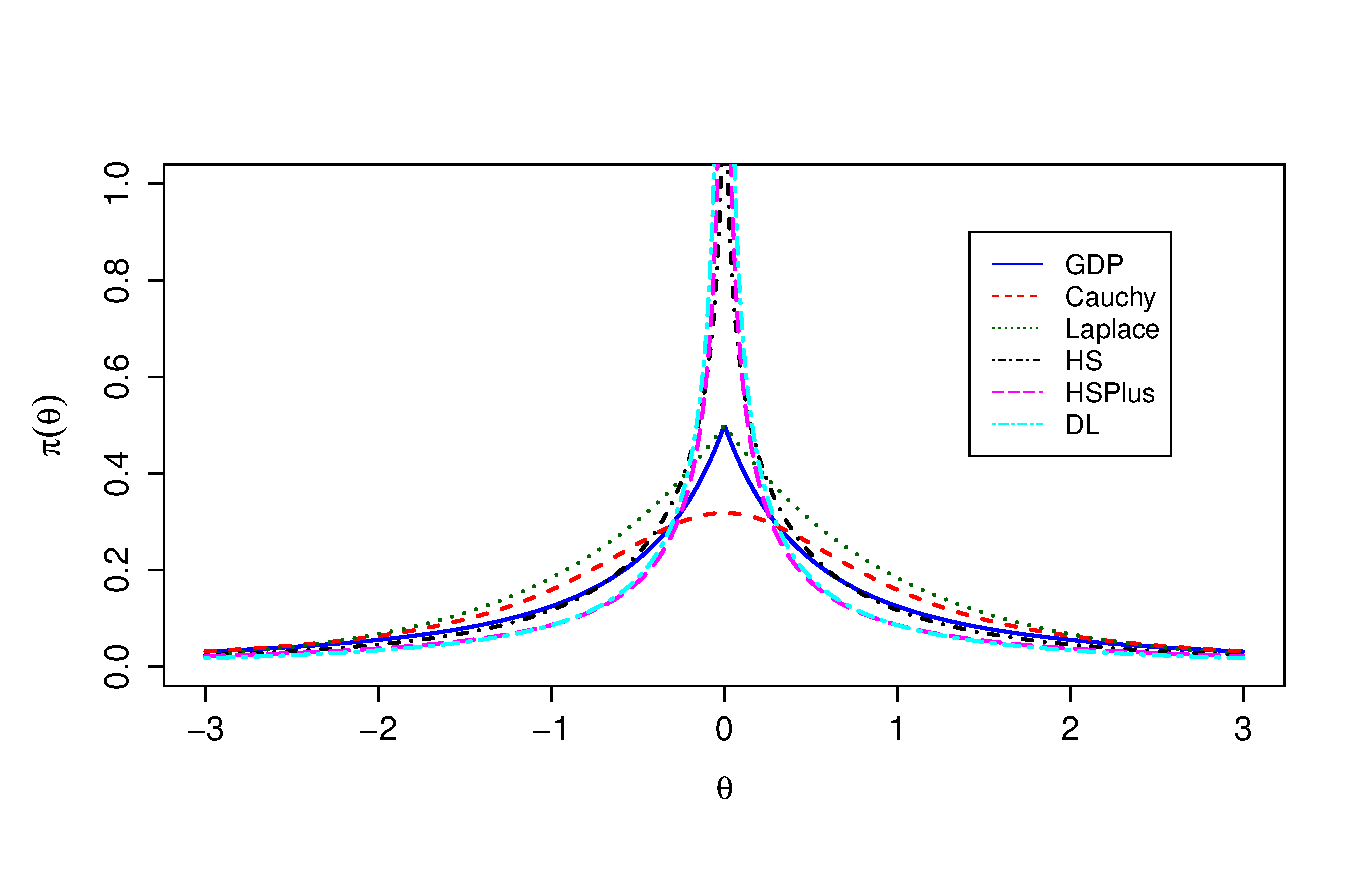
\includegraphics[height=2.5in,width=\textwidth]{densities_zero_new}%
%%	\caption{\footnotesize{Marginal prior densities near the origin. The legends denote the horseshoe+ (HSPlus), horseshoe (HS), Dirichlet-Laplace (DL), generalized double Pareto (GDP), Cauchy and Laplace priors.}}
	%\label{fig:zero}
	%\end{subfigure}
	%%\hspace{0.1in}
  %\begin{subfigure}[t]{0.45\linewidth}
	%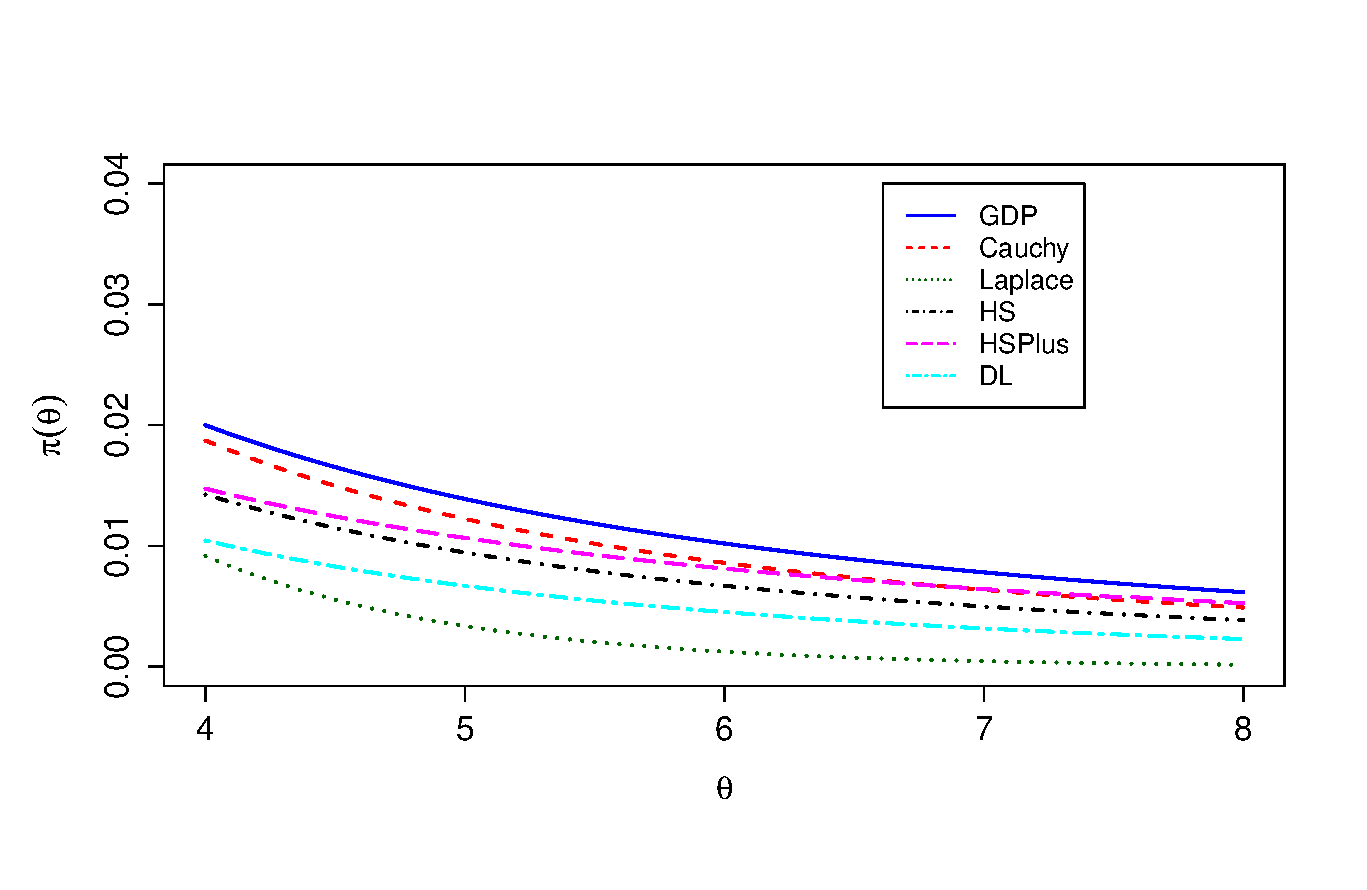
\includegraphics[height=2.5in,width=\textwidth]{densities_tails_new}
  %\label{fig:tails}
		%\end{subfigure}
 %\caption{Marginal prior densities near the origin (left) and in the tail regions (right). The legends denote the horseshoe+ (HSPlus), horseshoe (HS), Dirichlet-Laplace (DL), generalized double Pareto (GDP), Cauchy and Laplace priors.}
	%\label{fig:priors}
%\end{figure}

Now, we can Furthermore, using the representation of the \rm{DE} distribution as a scale mixture of Gaussians: 

\[
\beta_j \mid \phi , \tau \sim \text{\rm{DE}}(\phi_j \tau) \Rightarrow \left\{ \begin{array}{ccc}
\beta_j & \sim & \NormRV(0 , \psi_j\phi^2_j\tau^2); \\
\psi & \sim & \mathcal{E}\mathrm{xp}(1/2),
\end{array} \right. 
\] 

We get the augmented full hierarchical model :
\begin{align} \label{sq_dl_h}
[ \y \mid \bbeta, v^2 ] & \sim \NormRV(\X \bbeta, v^2 \I_n), \\
[\bbeta \mid \bphi, \tau , \bpsi ] & \sim \NormRV(\0, D_{\bpsi \bphi \tau}), \quad D_{\bpsi \bphi \tau} = \text{Diag}(\psi\phi_1^2\tau^2, \ldots, \psi\phi_p^2\tau^2), \\
\psi_j & \stackrel{iid}{\sim} \mathcal{E}\mathrm{xp}(1/2), \\
\bphi & \sim \text{\rm{Dir}}(a, \ldots ,a), \\
\frac{\tau}{v^2} & \sim \mathcal{G}\mathrm{amma}(pa , 1/2), \\
%[\lambda_1^2, \ldots, \lambda_p^2 \mid \tau^2] & \sim \prod_{j=1}^{p} \sim \frac{\tau^2}{2} e^{-%\lambda_j^2\tau^2/2} \d \lambda_j^2, \quad \lambda_j^2 > 0, \\
[v^2] & \sim \mathcal{G}\mathrm{amma}(\frac{n+1}{2} , 1/2).  
%[\tau^2] & \sim p(\tau^2) d\tau^2,  \; \tau^2 > 0. \quad [ \tau^2 \sim \GammaRV(r, \delta), \text{ or } \tau^2 \sim \CauchyRV(0,1). ]
\end{align}

%As we can see from Fig. \ref{fig:priors}, both the Horseshoe and the $\text{\rm{DL}}_a$ exhibit a singularity near zero. This marginal behavior at the origin guarantees sufficient prior mass near zero in order to accommodate for nearly black vectors. Furthermore, in the lower panel of Figure \ref{fig:priors}, we see a comparison of the tails of the different shrinkage priors. Unlike horseshoe and $\text{\rm{DL}}_a$, the Laplace prior does not have heavy tails that leave room for prior mass on possible high signal values. Hence we would expect the two former shrinkage priors to outperform the latter in both signal recovery and noise shrinkage. 


\section{Computation}\label{sec:comp}

%\subsection{Gibbs Sampler for \sql{}}\label{subsec:comp-sql}
%Let $ D_{\blambda} = \text{Diag}(\lambda_1^2, \ldots, \lambda_p^2)$ be the diagonal matrix of local shrinkage parameters. 
%Using the equivalent decomposition \eqref{eq:t_i}, and collecting the terms for $\bbeta$, the joint distribution can be re-written as follows with $t = 1/v^2$: 
%\begin{multline}
%f(\y, \bbeta, t, \blambda, \tau^2 \mid \r, \delta) \propto 
%\frac{1}{t^{3/2}} \exp\{-{1}/({2 t}) \} \exp \left[- \half \{ \bbeta^\T(\X^\T \X t + \D_{\blambda}^{-1})\bbeta - 2 \bbeta^\T \X^\T \y t \}\right] \\
%\prod_{i=1}^{p} {(\lambda_i^2)}^{-\half} \frac{\tau^2}{2} e^{-\lambda_i^2\tau^2/2} (\tau^2)^{r-1} e^{-\delta \tau^2} \label{eq:joint-beta}
%\end{multline}
%
%The full conditional distributions of $\bbeta$ and $\tau$ are easy to derive: The full conditional of $\bbeta$ is multivariate normal and $\tau$ is Gamma, exploiting the conjugacy. The parameters $t$ and $\lambda_i^2$ follow inverse Gaussian distribution, where we assume the following parametric form of the inverse Gaussian density:
%\[
%f(x \mid \lambda', \mu') = \sqrt{\frac{\lambda'}{2\pi}} x^{-3/2} \exp\left\{ - \frac{\lambda'(x-\mu')^2}{2(\mu')^2 x^2} \right \}, \quad x > 0 
%\]
%
%The full conditional distributions needed for implementing a Gibbs sampler are:	
%\begin{align*}
%\bbeta \mid \y, \blambda, t & \sim \NormRV \left( \A^{-1}\X^\T \y t , \A^{-1} \right), i = 1, \ldots, p, \\
%\text{ where } \A & = \X^\T \X t + \D_{\blambda}^{-1} \\
%t \mid \y, \bbeta & \sim \text{Inv-Gauss} \left(\mu' = {\norm{\y-\X\bbeta}_2}^{-1}, \lambda' = 1 \right) \\
%\lambda_i^{-2} \mid \beta_i, \tau & \sim \text{Inv-Gauss}(\mu' = \abs{\frac{\tau}{\beta_i}}, \lambda' = \tau^2)\\
%\tau^2 \mid \blambda, r, \delta & \sim \text{Gamma}(p + r, \delta + \sum_{i=1}^{p} \lambda_i^2/2)
%\end{align*}
%
%A special case of the linear regression model is the sparse normal means model: $y_i = \beta_i + \epsilon_i$, $\epsilon_i \sim \NormRV(0,\sigma^2)$, which results when the design matrix is equal to the identity matrix of appropriate dimension. The Gibbs sampler for the normal means model is identical to that for the linear regression, but faster as the full conditional distribution of $\beta_i$'s are univariate Gaussian, and hence more efficient than the multivariate sampling. 
%\beq \label{BSQ_NM}
%\beta_i \mid y_i, \lambda_i, t \sim \NormRV \left(y_i \frac{\lambda_i^2 t}{1 + t \lambda_i^2}, \frac{\lambda_i^2}{1 + t \lambda_i^2} \right), i = 1, \ldots, p.
%\eeq

\subsection{Gibbs Sampler for \sqdl{}}\label{subsec:comp-dl}

The hierarchical model for \sqdl{}, given in \eqref{sq_dl_h} exploits the Laplace Gaussian scale mixture and leads to straightforward posterior computations. To reduce autocorrelation, we rely on a blocked Gibbs sampler scheme. The sampler moves from the following blocks \rm{(i)} $ [ \bbeta \mid \bpsi , \bphi , \tau , \v^2 , \y ] $, \rm{(ii)} $[\bpsi \mid \bphi , \tau , \bbeta]$, \rm{(iii)}   $[ \bphi \mid \bbeta]$, \rm{(iv)} $[ \tau \mid \bphi, \bbeta, v^2 ]$, and \rm{(v)} $[ v^2 \mid \bbeta ,\tau , \y ]  $. Computing the full conditional distribution of the above blocks is standard and straightforward due to conjugacy except for the third block $[ \bphi \mid \bbeta]$. In their paper \citet{bhattacharya2014dirichlet}, developed a very efficient sampling scheme for this non-trivial step. We state the following result from their paper, for a complete proof see \citep{bhattacharya2014dirichlet}.


\begin{theorem}\label{dl_phi_post}
The joint posterior of $[\bphi \mid \bbeta ]$ has the same distribution as $ \left( T_1/T, \ldots \T_p/T \right)$, where $T_j$'s are independently distributed according to a \rm{gIG}$a-1 , 1 , 2\abs{\beta_j}$, and $T = \sum_{j=1}^{p}T_j$. 
\end{theorem}

Using the representation in Theorem \ref{dl_phi_post}, we get the following blocked Gibbs sampler:
\begin{itemize}
\item[(i)] Sample $[ \bbeta \mid \bpsi , \bphi , \tau , \v^2 , \y ]$ from $\NormRV \left( \bSigma \X^T\y/v^2 , \bSigma \right)$, with $$ \bSigma^{-1} = \frac{\X\X^T}{v^2} + \frac{\D^{-1}_{\bpsi \bphi^2}}{\tau^2} $$.

\item[(ii)]Conditional posterior of $[\bpsi \mid \bphi , \tau , \bbeta]$ can sampled in block  by independently drawing $ \psi_j \mid \phi_j , \tau , \beta_j $ from \rm{inv-Gaussian}$ (\frac{\phi_j\tau}{\abs{\beta_j}} ,1) $

\item[(iii)] Sample the conditional posterior of $[ \bphi \mid \bbeta]$ by drawing $ \ T_1, \ldots \T_p$ independently from \rm{gIG}$a-1 , 1 , 2\abs{\beta_j}$ and set $\phi_j = T_j/T$, with $T = \sum_{j=1}^{p}T_j$.

\item[(iv)] Sample $[ \tau \mid \bphi, \bbeta, v^2 ]$ from a \rm{gIG}$( pa-p , 1 , 2\sum^{p}_{j=1}\abs{\beta_j}/\phi_j )$ distribution.

\item[(v)] Sample $[ v^2 \mid \bbeta ,\tau , \y ]  $ by drawing $ \frac{1}{\sigma^2} $ from \rm{inv-Gaussian}$ ( [ \norm{\y - \X\bbeta} + \tau ]^{-1} ,1) $.
\end{itemize}

%\section{Marginal Density and Masreliez Theorem}
%\section{Posterior Properties}\label{sec:post-prop}
%\subsection{Shrinkage Characteristics of Bayes \sql{}}
%
%First, we compare the shrinkage profiles for the Bayesian \sql{} with that of the Horseshoe prior. Figure \ref{fig:profile} shows the posterior mean and median for the Bayesian \sql{} and Horseshoe prior plotted against the observations $y$. It appears from Fig. \ref{fig:profile} that the posterior mean estimator under the two methods behave almost identically, while the posterior median for Bayes-\sql{} offers a somewhat stronger shrinkage, resembling a hard-thresholding rule. 
%
%\begin{figure}[!ht]%
%\centering
%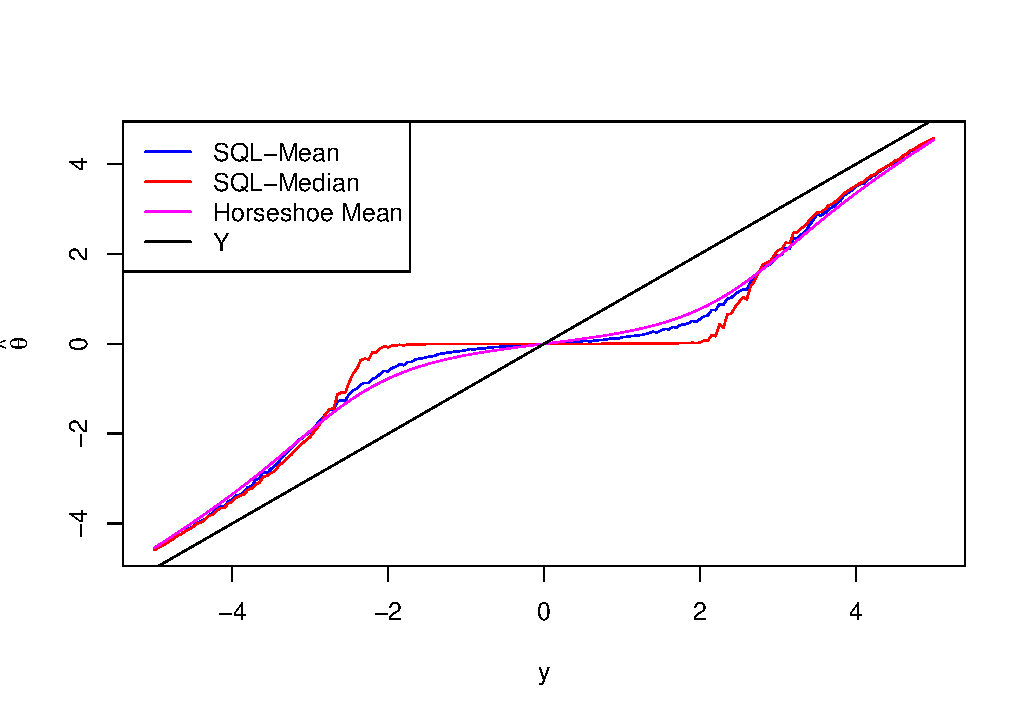
\includegraphics[width=0.7\columnwidth]{art/shrinkage_profile}%
%\caption{Shrinkage profile for the horseshoe posterior mean and Bayesian \sql{} posterior mean and median estimators. }%
%\label{fig:profile}%
%\end{figure}


\section{Simulation Studies}\label{sec:sim}

In this section, we investigate the performance of the methods proposed in \S \ref{ch:2} vis-a-vis the Lasso and other existing shrinkage priors. The criteria for comparison would involve finite sample performance of these methods in both estimation and model selection accuracy. In the latter case, we will also study the effect of column dependence of the design matrix that have been proven to affect model selection consistency in some methods. Before we illustrate the performance of the candidate priors, we begin by elucidating the usage of such priors for model selection in regression. 


\subsection{Different Variable Selection Strategies}\label{k-means}

The problem of variable selection and particularly in a "\textit{small n, large p}" setting has received quite some attention both from  the frequentist an Bayesian perspective. The Lasso, $\sqrt{\text{\rm{Lasso}}}$, horseshoe, Dirichlet-Laplace and numerous other methods were in part developed to tackle this problem. While the frequentist methods usually yield a sparse estimate, that is the estimated $\hat{\bbeta}$ vector has entries that are exactly zero, their Bayesian counterparts always require a decision rule to classify an estimated coefficient as either zero or not. As we discussed in \S \textbf{2.6.2}, decision rules for the horseshoe have already been studied, and shown to be optimal under some conditions for the normal means problem and regression settings where the design matrix is orthogonal. Likewise, for the Bayesian shrinkage priors considered in this work, we need a method to decide whether a coefficient should be classified as signal or noise. Such decision rule, can also be viewed as a variable selection step, given that any covariate for which the coefficient has been classified as zero is thrown out of the model. In this work, we decided to look at the posterior sample means of the $\hat{\bbeta}$ vector, and apply a k-means clustering on $\abs{\hat{\beta_j}} $ with only two cluster centers. We expect two clusters centers, one concentrated around zero for the noise signals and one away from zero. This method is motivated by the assumption that the true parameter vector is generated according to a two groups model. That is, each $\beta_i$ is generated from : 
\[
\beta_i \sim \tfrac{q}{p} \delta_{A} + \tfrac{p-q}{p} \delta_{0}, \ \text{so that }  \bbeta = ( \underbrace{ A, \ldots ,A}_{q}, \overbrace{0, \ldots 0}^{p-q} ) 
\]

After clustering the posterior mean vector, we classify the $\beta$'s according to the following steps : 
\ben
\item[1-] We look first at the two cluster centers $\left\lbrace \c_1 , \c_2 \right\rbrace $, and compare them in absolute value. Let $\C_s = max\left\lbrace \c_1 , \c_2 \right\rbrace$ and $\c_n = min\left\lbrace \c_1 , \c_2 \right\rbrace$. So that the $\c_s$ is the cluster center of the signals while $\c_n$ for the noise.
\item[2-] For all $\hat{\beta_j}$, look at the corresponding cluster, if $\abs{\hat{\beta_j}} \in \c_n $, then $\hat{\beta}_j^{dec}= 0$. Otherwise, $\hat{\beta}_j^{dec} = \hat{\beta_j}$.
\item[3-] Our final estimated coefficient vector is $\hat{\bbeta}^{dec} = \left\lbrace \hat{\beta}^{dec}_{j} \right\rbrace_{1\leq j \leq p}$.
\een

Clearly, unlike $\hat{\bbeta}$, which will never have exactly zero entries, the new $\hat{\bbeta}^{dec}$ given by the above described decision rule shrinks the noise coefficients to exactly zero, hence performing a variable selection. In this work, we stick to the case of the two groups model. However, the k-means method can be extended to a wider class of models. In fact, \citet{li2017variable} suggested a sequential $2$-means clustering algorithm in case the model presents signals of varying strength level.

One of the many interesting questions that arise with variable selection, is \textit{model selection consistency}. This property essentially means that the method used consistently selects the true model. It should be emphasized that model selection consistency and estimator consistency are entirely two different properties. Recall that estimator consistency holds if and only if:
\[ 
\hat{\bbeta}^{n} -  \bbeta \stackrel{\P}{\to}0, \ \text{as } n \to \infty, 
\]
while model selection consistency requires:
\[ 
\P\left[ \lbrace i : \hat{\beta}_i^{n} \neq 0 \rbrace = \lbrace i : \beta_i \neq 0\rbrace \right] \to 1, \ \text{as } n\to\infty. 
\]

\subsection{Effect of Dependence}

The optimality properties of Lasso are well-known and they depend on ``neighborhood stability'' or ``irrepresentability'' condition and ``beta-min'' condition. Informally, these conditions guarantee against ill-posed design matrix and separability of signal and noise parameters. We show here a small simulation study inspired from Zhao et al.[2006] to show that the effect of `irrepresentability condition' is not as strong on our methods as it is on the Lasso.

We describe the ``irrepresentable" condition below:\par Suppose, the sample covariance matrix is denoted by $\hat{\Sigma} = nX^T X$ and the active-set $S_0 = { j : \beta_j \neq 0}$ consists of first $s_0$ elements of $\beta$. One can partition the $\hat{\Sigma}$ matrix as

$$ \hat{\Sigma} = \left(\begin{array}{cc}
\hat{\Sigma}{s_0,s_0} & \hat{\Sigma}{s_0,p-s_0} \\ \hat{\Sigma}{p-s_0,s_0} & \hat{\Sigma}{p-s_0,p-s_0} \end{array} \right) $$

where $\hat{\Sigma}_{s_0,s_0}$ is a $s_0\times s_0$ matrix corresponding to the active variables and so on. The irrepresentable condition for variable selection consistency of Lasso is:

$$ \vectornorm{\hat{\Sigma}{p-s_0,s_0} \hat{\Sigma}{s_0,s_0}^{-1} sign(\beta_{S_0})}_{\infty} \leq \theta \quad \mbox{ for some } 0 < \theta < 1 .$$

This condition is sufficient and almost necessary in the sense that the necessary condition is only slightly weaker than the sufficient condition. The necssary condition requires '$\leq 1$', while the sufficient condition involves $\leq \theta$ for some $0 < \theta < 1$. The irrepresentable condition fails to hold if the design matrix is too ill-posed, i.e. has multi-collinearity.

\citep{buhlmann2011statistics} warn the readers that the irrepresentable condition may fail even though the design matrix is not ill-posed and it might restrict what can be done in high-dimensional problems. Zhao et al. (2006) provide numerical example to show the effect of the irrepresentable condition on the variable selection performance of Lasso. They showed that the probability of selecting the true sparse model is an increasing function of the irrepresentability condition number, defined as $$ \eta_{\infty} = 1 - \vectornorm{ \hat{\Sigma}{p-s_0,s_0} \hat{\Sigma}{s_0,s_0}^{-1} sign(\beta_{S_0}) }_{\infty} . $$ In particular, the probability of Lasso selecting the true model is almost 1 when $n_{\infty} > 0.2$ and it is almost zero when $\eta_{\infty} < -0.3$.

We simulated data with $n = 100, p = 60$ and $q = 7$ with the sparse coefficient vector $\beta_{q}^* = (7,5,5,4,4,3,3)^T$, $\sigma^2$ was set to $5$ to allow for heavy tailed data. Like Zhao et al. (2006) we first draw the covariance matrix $\Sigma$ from $Wishart(p, I_p)$ and then generate design matrix $X$ from $N(0,\Sigma)$. This design is repeated a $100$ times, and at each iteration we apply the Lasso, horseshoe, Bayesian-$\sqrt{\text{Lasso}}$ and the $\sqrt{\text{\rm{DL}}}$ 100 times to each of the $100$ generated models. For the three Bayesian methods we run the Markov Chain for 9000 samples, discarding the first 1000 thousand as a burn-in step and finally thinning every two samples. We select the posterior median and then apply a variable selection step. For the horseshoe, we take advantage of the credible set properties and use them to classify the $\beta_j$'s. For the other two methods discussed in this work, we implement the k-means clustering procedure discussed in Subsection \ref{k-means}. The Lasso automatically yields sparse vector estimates, we only need to select the tuning parameter $\lambda$, which represents the penalty level, we set $\lambda$ to the value that minimizes the MSE based on a 10 fold cross validation.

The goal of this simulation study is to observe the effect of the irrepresentability condition on our proposed methods and compare them to the Lasso and horseshoe. We are particularly interested in model selection consistency, so we look at the proportion of correctly selected models out of the 100 replicates for each design.

\citet{zhao2006model} showed that the irrepresentability condition may not hold for such a design matrix. In fact, in our simulation studies the $\eta_\infty$'s for the 100 simulated designs were between $[-1.02, 0.36]$. We expect the Lasso to perform well when $\eta_\infty>0$ and poorly when $\eta_\infty<0$. We generate $n = 100$ design matrices and for each design, 100 simulations were conducted by generating the noise vector from $\NormRV(0, \sigma^2 I)$.

Figure \ref{fig:profile:MSP_irrep} below shows the percentage of correctly selected model as a function of the irrepresentable condition number, $\eta_\infty$ for Lasso,the Horseshoe prior, the Bayesian-\sql{} and the \sqdl{}.

As expected, Lasso's variable selection performance is crucially dependent on the irrepresentability condition but the Horseshoe prior almost always recovers the true sparse $\beta$ vector irrespective of $\eta_\infty$. Strikingly, both our methods succeed in always recovering the true model. This strong performance independently of  $\eta_\infty$, clearly presents an advantage and is worth studying from a theoretical view point.

\begin{figure}[ht!]%
\centering
%\vspace{0.1in}
\begin{subfigure}[t]{0.45\textwidth}
\centering
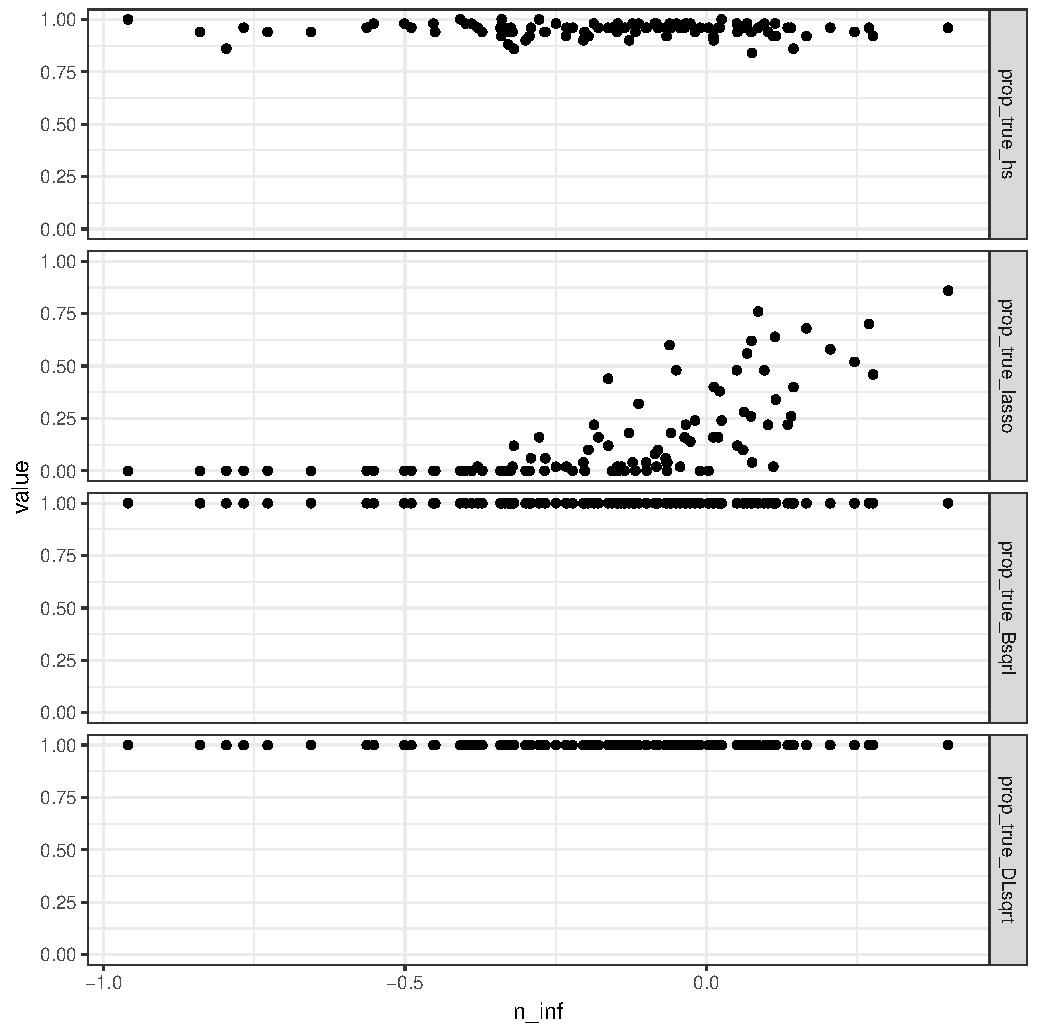
\includegraphics[width=\columnwidth]{Irrep_model_selec_n100p60_q50_2groups}%
\caption{Effect of $\eta_{\infty}$ on model selection}%
\label{fig:profile:MSP_irrep}%
\end{subfigure}
\begin{subfigure}[t]{0.45\textwidth}
\centering
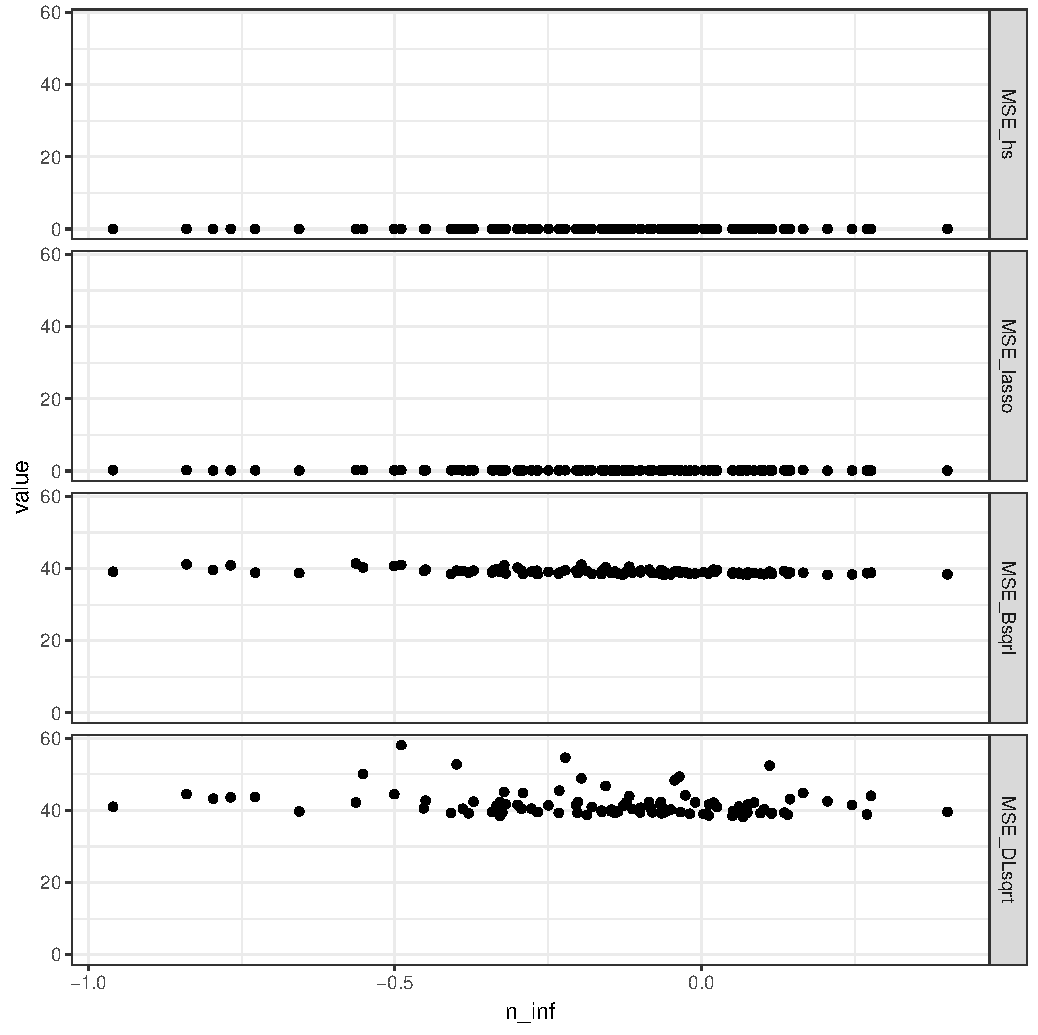
\includegraphics[width=\columnwidth]{Irrep_MSE_selec_n100p60_q50_2groups}%
\caption{Effect of  $\eta_{\infty}$ on the MSE}%
\label{fig:profile:MSE_irrep}%
\end{subfigure}
\caption{Effect of Irrepresentability Condition on model selection and estimation error for different shrinkage estimators}
\label{fig:profile}
\end{figure}

Given that the values of the non-zero entries of the true $\bbeta$, do not differ much in magnitude, we think that this excellent performance in terms of variable selection, is in part due to the 2-means clustering procedure. 

In Fig. \ref{fig:profile:MSE_irrep}, we see the evolution of the MSE calculated over the replicated samples for each design matrix. A surprising results, that we observe, is the pronounced difference from the model selection summary in figure \ref{fig:profile:MSP_irrep}. Note, however that the MSE computed here is for the posterior median before any decision rule has been applied. Since the Bayesian methods do not provide exact sparse estimates, there will be an added error component wise across the whole $\bbeta$ vector. Having a moderately large $p$, thus increases this error proportionally. Interestingly, the lasso despite not selecting the true model in approximately all designs, shows a very low MSE. This can be explained in part by the exact zero estimator yielded by this method, coupled with the sparse nature of the underlying true vector. Horseshoe, remarkably performs very well in terms of both true model selection and low MSE. Given that it is a Bayesian method, hence returning no exact zero entries, its impressive performance indicates both a very low bias for all components as well as small empirical variance of the posterior median.


It is also important to note how this simulation study provides a clear separation and points out the difference between model selection consistency and estimation consistency. As pointed out in the beginning of this section, the two properties are different and somehow counter-intuitively none of them implies the other. In Fig. \ref{fig:profile:MSE_irrep} we see how lasso has very low MSE, which suggest estimator consistency, while Fig. \ref{fig:profile:MSP_irrep} clearly shows that lasso does not enjoy model selection consistency. Conversely, both \sql and \sqdl successfully capture the true model independently from $\eta_{\infty}$, but at the same time shows high values of MSE.


%\subsection{Effect of Mutual Coherence Condition}

\subsection{Adapting to Sparsity levels}

Most penalized regression methods, and shrinkage priors operate under the assumption that the parameter of interest is sparse in some sense. In addition, the widespread attention that these methods have received in the past decade was mostly focused on theoretical properties in the case of sparse models. Although, sparsity or parsimony of statistical models is crucial for their proper interpretations, as in sciences
and social sciences, we should address the cases where true coefficient vectors, have zero entries but are not completely sparse. Furthermore, the case of nearly black vectors has been investigated thoroughly, yet little attention has been given to adaptability to varying degrees of sparsity. In this section, we try to address this issue by running simulations on model designs with varying underlying levels of sparsity. Like the previous section, we will compare our methods to Lasso the gold standard for best subset selection of predictors, and the horseshoe prior which is a state-of-the-art Bayesian estimator for sparse signals. We will focus on misclassification probability and MSE as indicators of method performance. We limit ourselves to the case of two group generating model for model parameters. 

We simulated data with $n = p = 100$, the entries of the design matrix $\X$ were simulated from a $\NormRV(0 ,2)$ distribution, with the error variance set to $\sigma^2 = 5 $. We sampled $100$ different design matrices, and for each of these design matrices, we applied the four different methods with varying degrees of sparsity. That is for each of the $100$ designs, say $\X$, we have nine different response vectors obeying the following equation:
\beq\label{sparsity_mod}
\y^{k} = \X \bbeta^{k} + \bepsilon, \ \text{where } \bbeta^{k} =  ( \underbrace{ 5, \ldots ,5}_{q = k\nicefrac{p}{10}}, \overbrace{0, \ldots 0}^{p-q} ) \ \text{for } k = 1,\ldots, 9 .
\eeq

Hence for each sparsity level, we have a $100$ replicates, from which we compute the misclassification proportion, that is the number of times a given method does not select the true model, and the MSE. Here we also compute for the Bayesian methods, the MSE after the decision rule was performed $\textbf{\rm{MSE}}(\hat{\bbeta}^{dec})$. Table \ref{table:msp}, \ref{MSE_dec} and \ref{MSE} summarize the numerical results for varying levels of sparsity. 


\begin{table}[h!]
\caption{Misclassification proportion \\ according to sparsity}\label{table:msp}
\begin{center}
\footnotesize{
\begin{tabular}{c|c|c|c|c|c|c|c|c|c|}
\cline{2-10}
    & 0.1  &  0.2  &  0.3  &  0.4  &  0.5 &   0.6  &  0.7  &  0.8 &   0.9 	\\
\hline
\multicolumn{1}{|r|}{Lasso} &  0.2306 & 0.2786 & 0.2481 & 0.2250 & 0.2241 & 0.2225 & 0.2087 & 0.1829 & 0.1782	\\
\hline
\multicolumn{1}{|r|}{Horseshoe} &  0.0013 & 0.0041 & 0.0094 & 0.0077 & 0.0011 & 0.1015 & 0.5747 & 0.7140 & 0.8210\\
\hline
\multicolumn{1}{|r|}{B-\sql} & 0.0000 & 0.0006 & 0.0040 & 0.0201 & 0.0569 & 0.1261 & 0.2054 & 0.3124 & 0.4414 \\
\hline
\multicolumn{1}{|r|}{\sqdl} & 0.0000 & 0.0004 & 0.0008 & 0.0022 & 0.0043 & 0.0091 & 0.0134 & 0.0201 & 0.0577 \\
\hline
\end{tabular}}
\end{center}

\end{table}

From Table \ref{table:msp}, we see that Lasso never selects the true model, and on average misses $20 \% $ of the coefficients. The horseshoe does well when the sparsity  level is very low, this is well in accordance with the theoretical results for horseshoe's performance in the case of nearly black vectors. The Bayesian \sql, does almost as well as the horseshoe in terms of misclassification probability in the case of sparse parameters. However, both methods seem to break down when the proportion of non-zero parameters increases, i.e. when we shift from a sparse regime to a dense regime. The \sqdl escapes this problem and seems totally oblivious to sparsity level. This method almost pinpoints the true model in all cases. Figure \ref{fig:msp}, gives a better comparison than the above table, we can see clearly how the misclassification proportion for the horseshoe and Bayesian \sql are affected by sparsity levels, and how \sqdl adapts easily to that level. This suggests that the added global shrinkage parameter in \sqdl  successfully adapts to the sparsity level of the $\bbeta$ vector. 

Likewise, from Tables \ref{MSE_dec} and \ref{MSE} , we can see how the MSE for all four methods is affected by sparsity level. Note that for Table \ref{MSE_dec}, the MSE was computed after a classification step was applied to the original Bayesian estimates, that is the estimates will have zero values for parameters that were not classified as signals. This is similar to the half-thresholding estimates of \cite{tang2016bayesian}, but here we apply the idea to a general shrinkage estimator. Lasso and horseshoe exhibit a better MSE in sparse settings, but their MSE increases drastically, whenever the number of non-zero parameters increases and the sparsity level crosses a certain threshold. The Bayesian-\sql, and the \sqdl have higher MSE values, however after classifying the parameters the MSE decreases significantly. 



\begin{table}[h!]
\caption{MSE according to sparsity\\ after applying a decision rule}\label{MSE_dec}
\begin{center}
\footnotesize{
\begin{tabular}{c|c|c|c|c|c|c|c|c|c|}
\cline{2-10}
    & 0.1  &  0.2  &  0.3  &  0.4  &  0.5 &   0.6  &  0.7  &  0.8 &   0.9 	\\
\hline
\multicolumn{1}{|r|}{Lasso} & 1.29 &  2.69 &  6.18 &  17.07 & 66.76 &  241.71 & 472.8 &  679.67 &  922.11	\\
\hline
\multicolumn{1}{|r|}{Horseshoe} &   0.33 & 0.95 &  2.31 &  3.83 &   5.27 &   268.69 & 1509.02 & 1883.04 & 2177.61 \\
\hline
\multicolumn{1}{|r|}{B-\sql} & 8.68 & 20.95 & 47.49 & 101.59 & 203.84 & 378.51 & 579.83 &  856.5 &   1193.86 \\
\hline
\multicolumn{1}{|r|}{\sqdl} &4.1 &  9.97 &  17.5 &  28.2 &   40.83 &  63.65 &  81.59 &   107.83 &  201.22 \\
\hline
\end{tabular}}
\end{center}

\end{table}

\begin{figure}[ht!]
\centering
\begin{subfigure}[t]{0.8\linewidth}
\centering
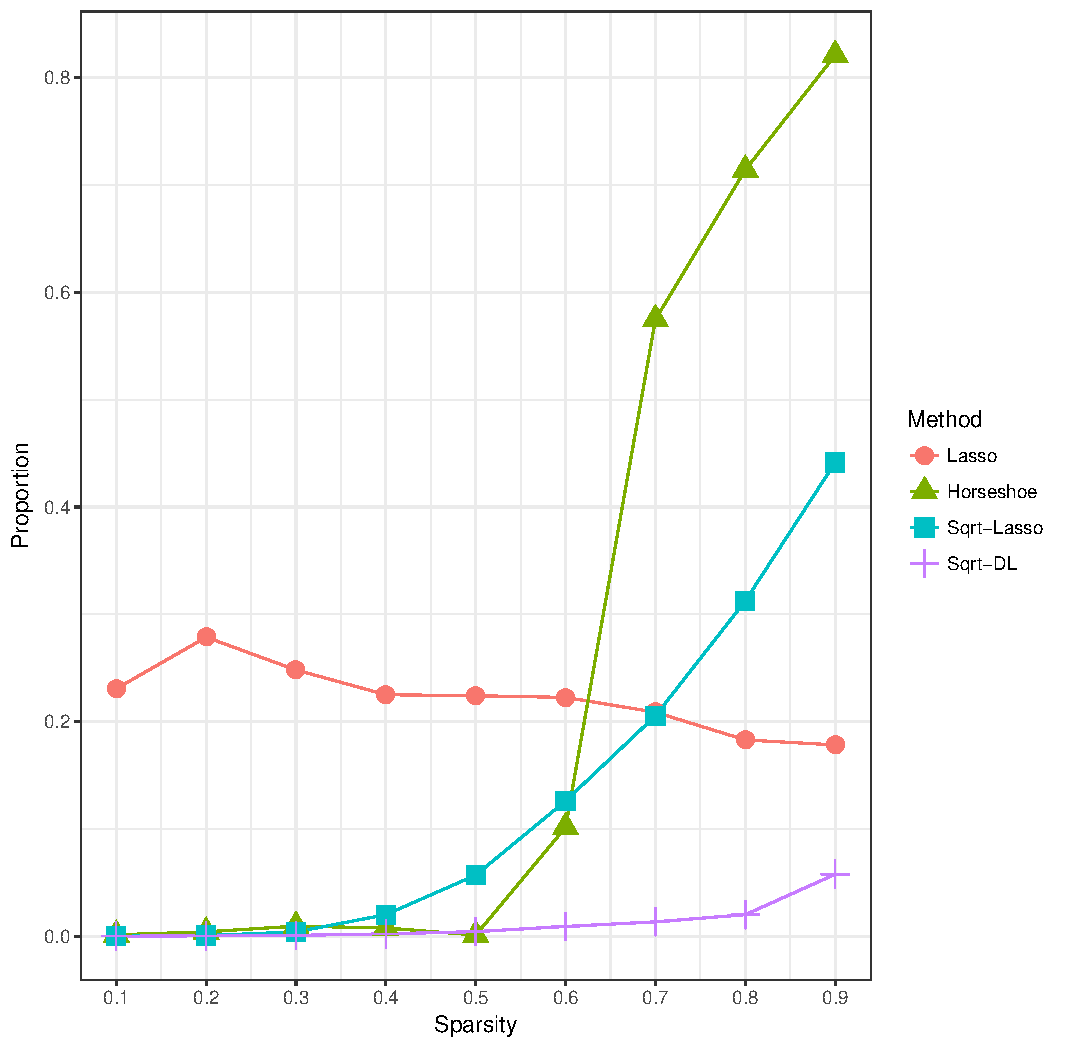
\includegraphics[height = 2in, width =\linewidth]{Sparsity_MSP_n=p}
\caption{Misclassification proportion as a function of sparsity level.}
\label{fig:msp}

\end{subfigure}
\begin{subfigure}[t]{0.8\linewidth}
  \centering
  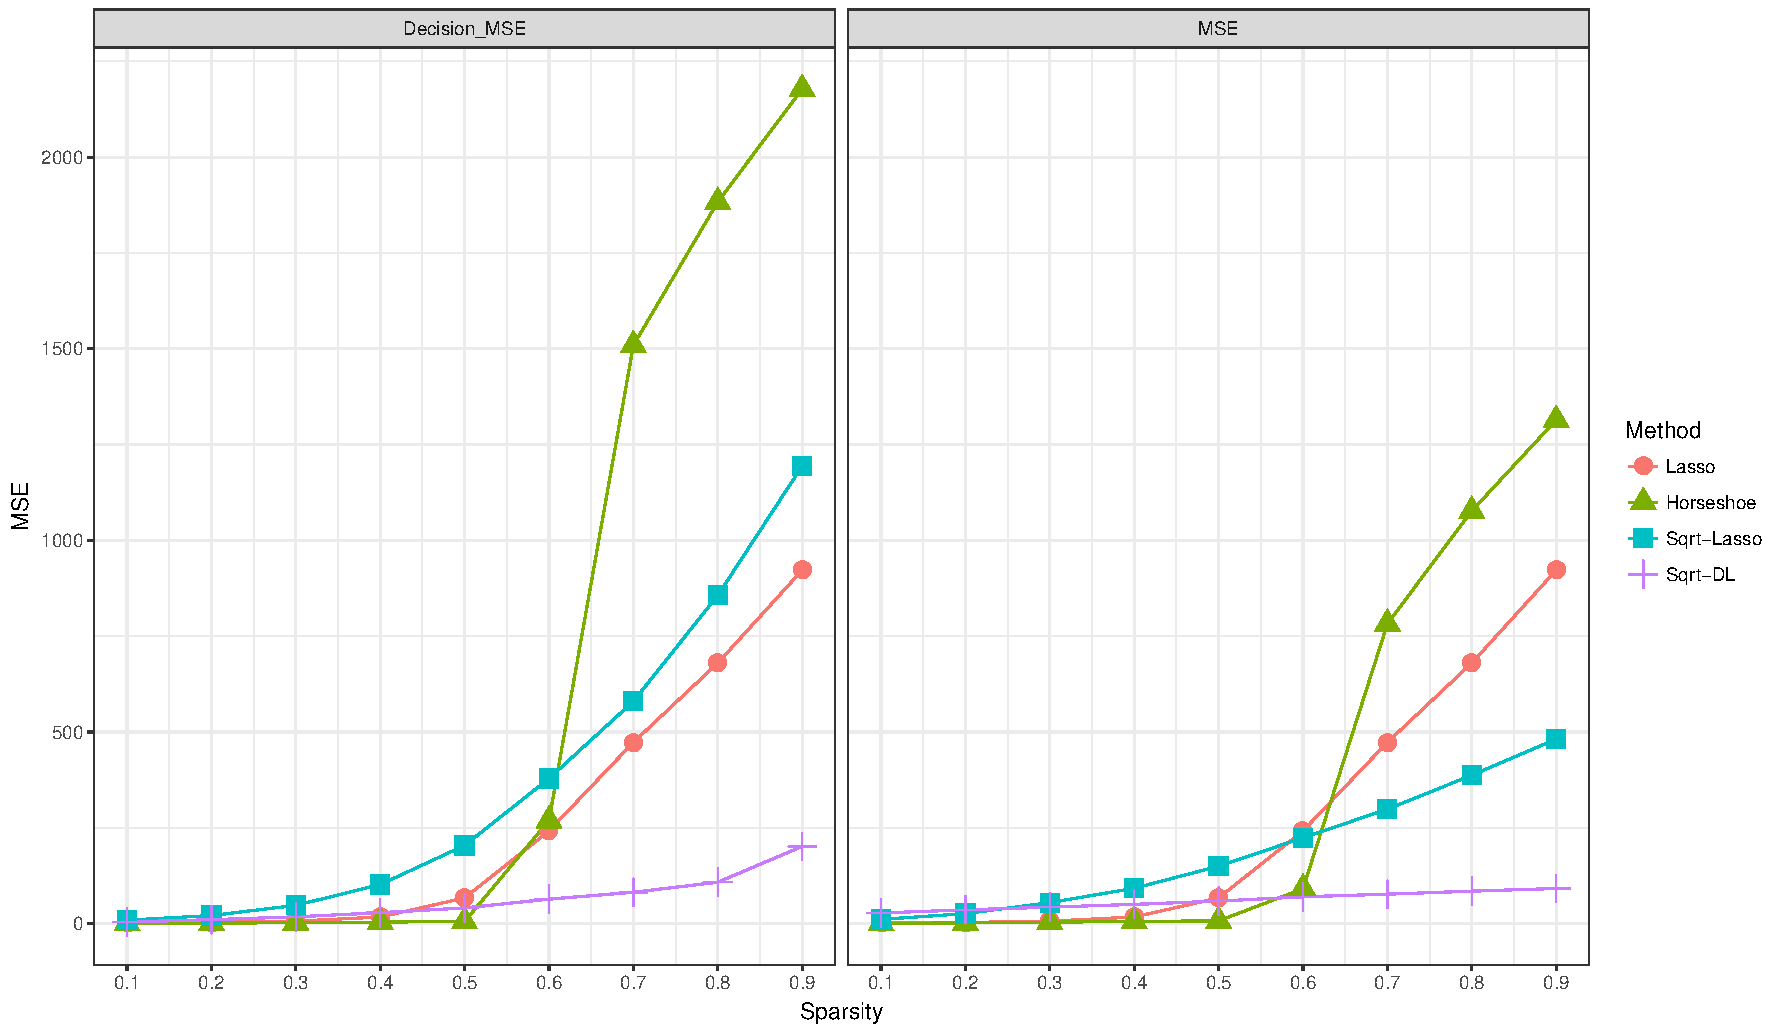
\includegraphics[height = 2in, width=\linewidth]{Sparsity_MSE_high_n=p}\caption{A comparison of the MSE as a function of sparsity level}
\label{fig:test}
\end{subfigure}
\caption{Effect of changing sparsity levels on model selection and estimation}
\label{fig:sparsity}
\end{figure}


\begin{table}[h!]
\caption{MSE according to sparsity}\label{MSE}
\begin{center}
\footnotesize{
\begin{tabular}{c|c|c|c|c|c|c|c|c|c|}
\cline{2-10}
    & 0.1  &  0.2  &  0.3  &  0.4  &  0.5 &   0.6  &  0.7  &  0.8 &   0.9 	\\
\hline
\multicolumn{1}{|r|}{Lasso} & 1.29 &  2.69 &  6.18 &  17.07 & 66.76 &  241.71 & 472.8 &  679.67 &  922.11	\\
\hline
\multicolumn{1}{|r|}{Horseshoe} &   0.5 &   1.49 &  3.55 &  5.56 &  6.96 &   90.73 &  782.25 & 1076.87 & 1313.92 \\
\hline
\multicolumn{1}{|r|}{B-\sql} & 10.74 & 26 &    54.59 & 92.16 & 149.51 & 223.96 & 298.3 &  387.07 &  481.41 \\
\hline
\multicolumn{1}{|r|}{\sqdl} & 27.63 & 35.65 & 42.76 & 50.06 & 58.48 &  69.78 &  76.6 &   84.56 &   91.42 \\
\hline
\end{tabular}}
\end{center}
\end{table}



%\begin{figure}[!h]%
%\centering
%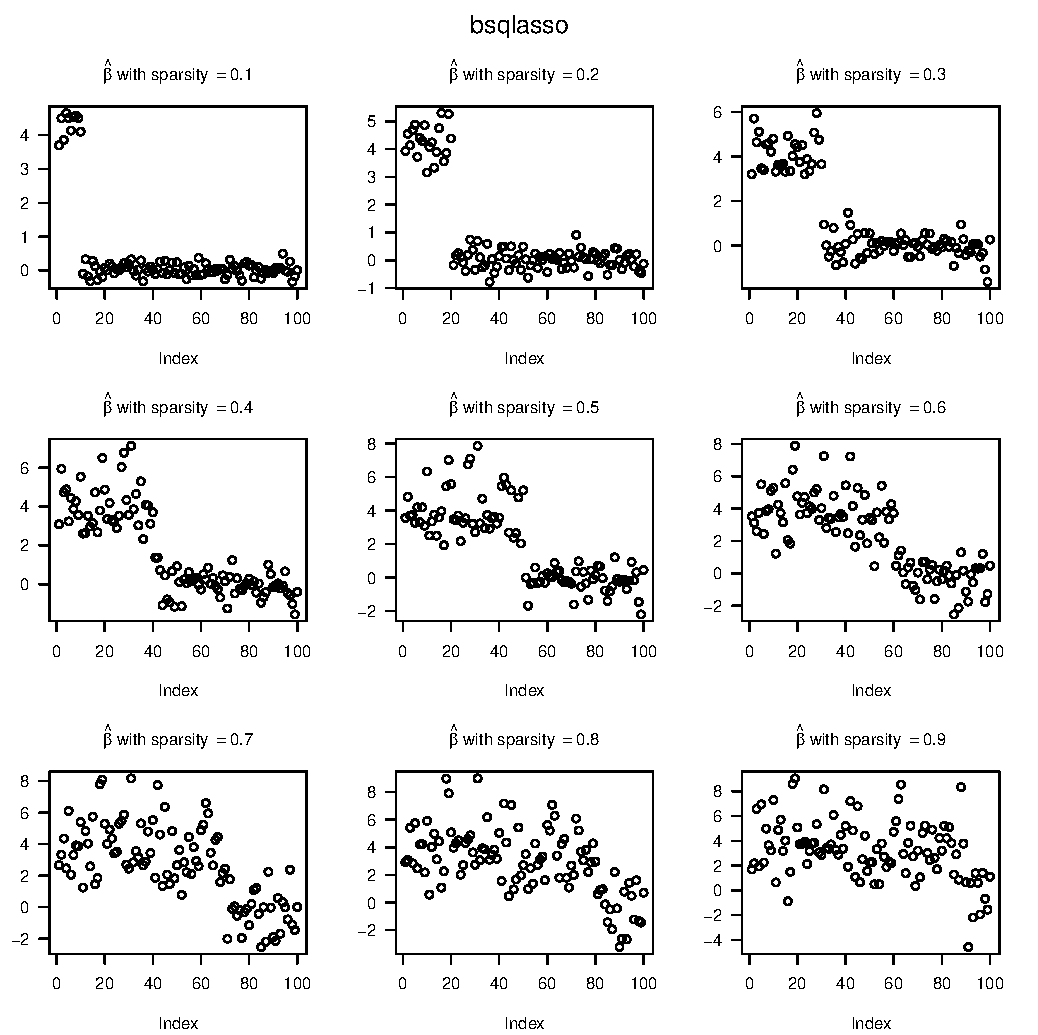
\includegraphics[width=0.9\textwidth , height = .8\textheight]{Sparsity_Bsql}%
%\caption{Adapting to sparsity level Bsql }%
%%\label{fig:profile}%
%\end{figure}
%
%\begin{figure}[!h]%
%\centering
%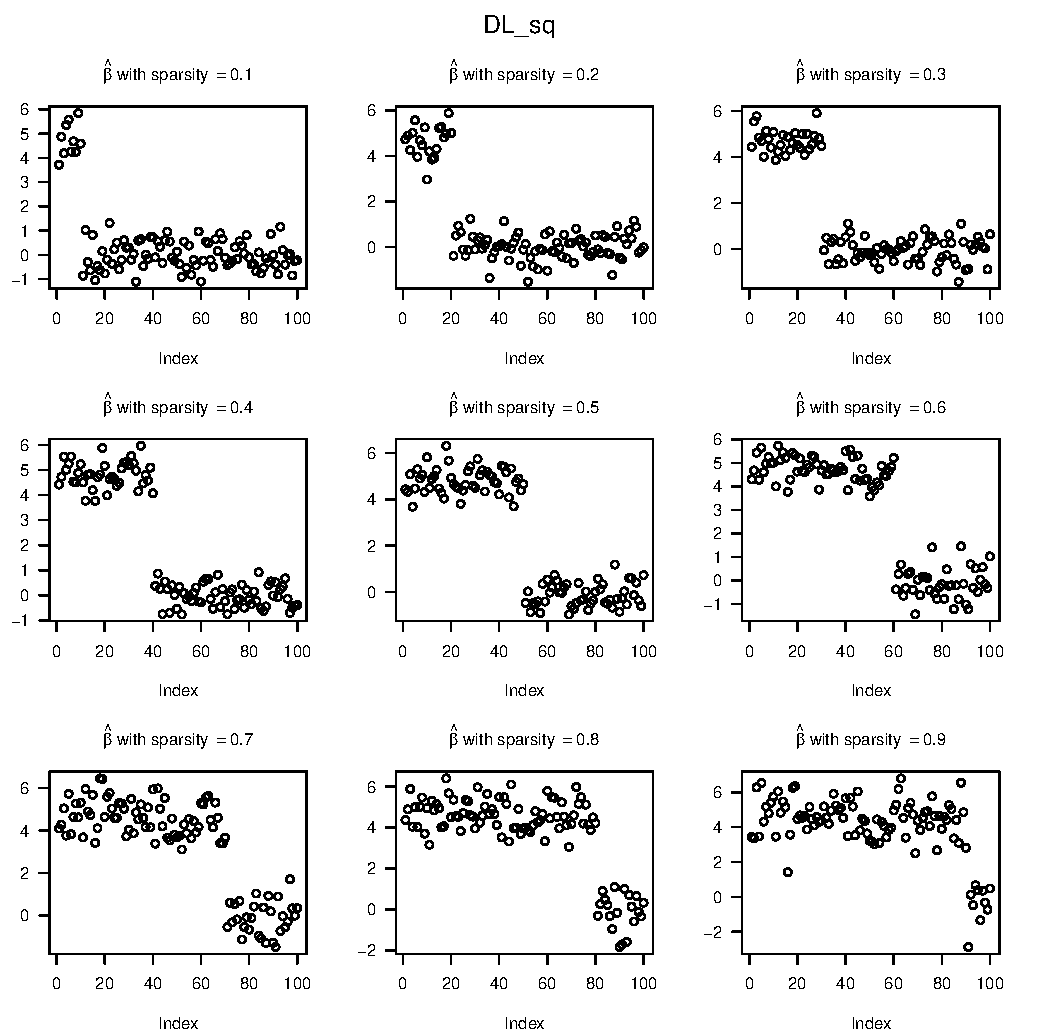
\includegraphics[width=0.9\textwidth , height = .8\textheight]{Sparsity_DL_sq}%
%\caption{Adapting to sparsity level DLsq }%
%%\label{fig:profile}%
%\end{figure}


%\section{Theoretical Results}

\section{Discussion and Future Directions}\label{sec:future}

In this work, we first developed a Bayesian representation of the \sql, taking advantage of normal scale mixture representation of the Laplace prior, we were able to develop a Gibbs sampler for the parameters of the model. Numerical results showed satisfactory performance in the case of sparse normal means and high dimensional regression. Furthermore, unlike the horseshoe and other global local shrinkage priors, this method obviates the need to learn, scale or estimate the precision parameter $\sigma$. We also found that a k-means classification step on the posterior estimates of the parameter vector outperforms other decision rules like the use of credible intervals for horseshoe. 

Motivated by the strong properties of global local shrinkage priors, specifically, their singularities at zero and their ability to concentrate at near minimax rate, we added a global component to our model. This ensured, that the new prior placed sufficient mass around the origin, thus a-priori favoring nearly black sets, yet we did not observe any improvement in concentration coverage, as the MSE stayed quite high in our empirical investigation. Surprisingly, the effect of the added global parameter was a nice adaptability to sparsity levels. This new interesting property requires more theoretical investigation. 
%\item Theoretical Justification for sparsity and dependence
To show how the global parameter adapts to sparsity level, we conducted a small experiment, where models with different proportions of non-zero parameters were constructed, and we implemented both the \sqdl and the horseshoe. Here we are only interested in the effect of different sparsity levels on $\btau$. In Fig. \ref{fig:tau-hs}, we see how in the case of the horseshoe the boxplots for the $\btau$ samples continue to increase until we reach  level of approximately $.5$ where a dramatic breakdown happens. Clearly, in the left side of the figure, we can say that $\btau$ follows the monotone increase in the proportion of non-zero parameters, but when this proportion approaches and exceeds the $.5$ threshold, the method is no longer able to follow and adapt the sparsity level. This behavior also explains why the MSE and the proportion of misclassified $\beta$'s exploded whenever the proportion of non-zero $\beta$'s exceeded the threshold of $0.5$, as shown in Fig \ref{fig:msp} and Fig. \ref{fig:test}.


On the other hand, we also saw in Fig \ref{fig:msp} and Fig. \ref{fig:test}, how the \sqdl performance remained satisfactory and was in no way affected by changes in the sparsity level. The boxplots of $\btau$ samples in Fig. \ref{fig:tau-dl}, back up our conjecture, unlike the horseshoe, here the global shrinkage parameter follows and learns correctly the degree of sparsity. In the future, we would like to theoretically investigate this claim and try to prove it.

\begin{figure}[ht!]%
\begin{subfigure}{0.48\linewidth}
\centering
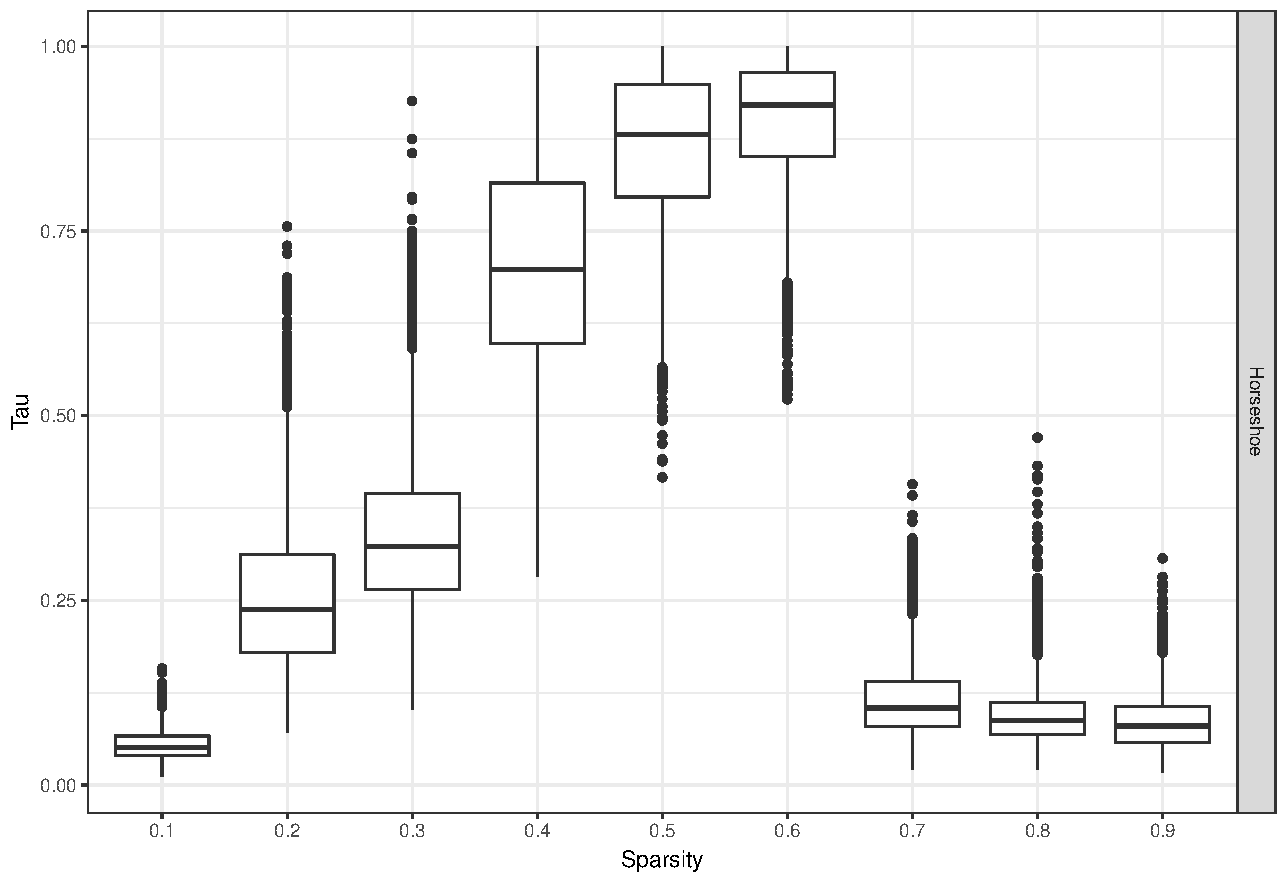
\includegraphics[height=2in]{Tau_hs}\caption{Evolution of $\btau$ on terms of sparsity level for the Horseshoe method}
\label{fig:tau-hs}
\end{subfigure}
\begin{subfigure}{0.48\linewidth}
\centering
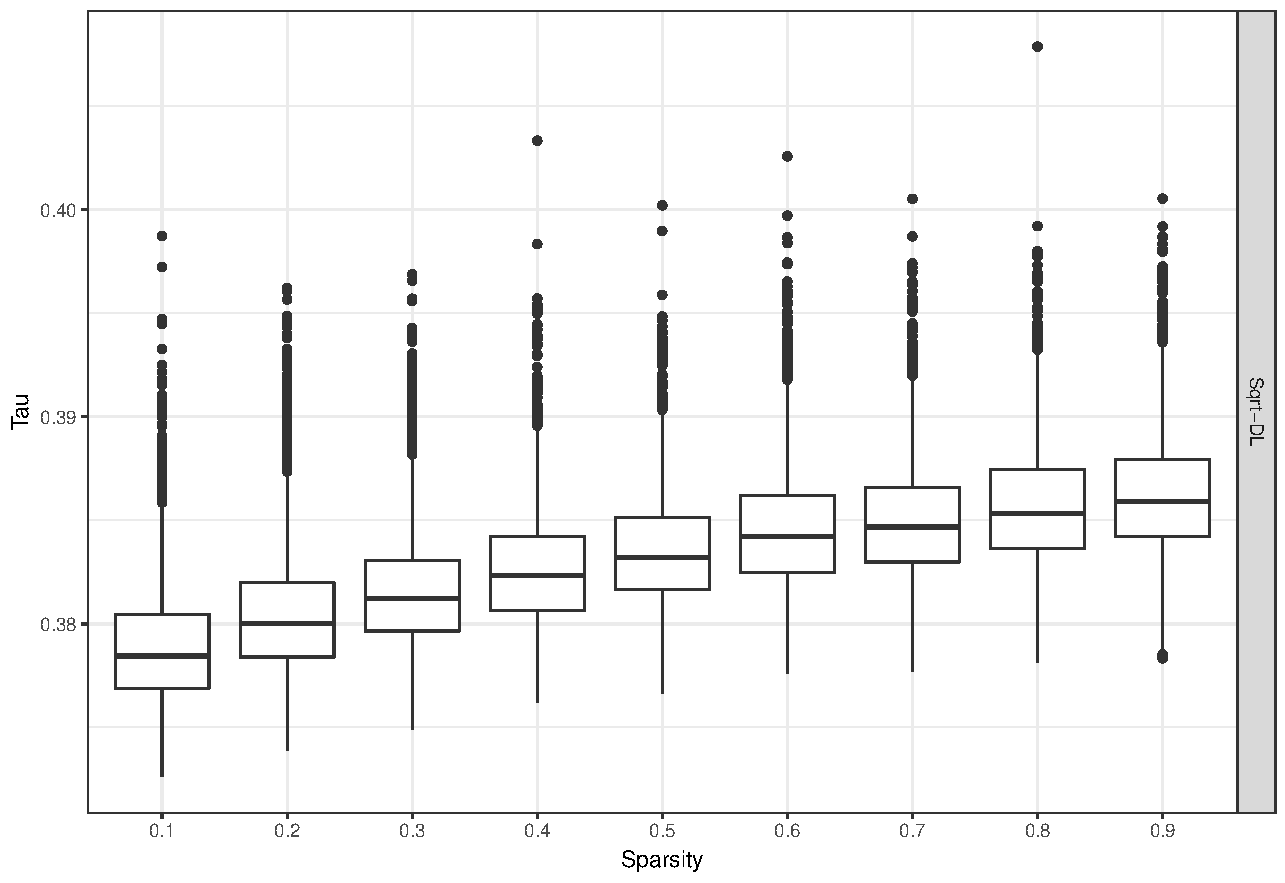
\includegraphics[height=2in]{Tau_dl}\caption{Evolution of $\btau$ on terms of sparsity level for the \sqdl method}
\label{fig:tau-dl}
\end{subfigure}
\caption{Adaptivity of $\tau$ for different shrinkage priors.}%
\label{fig:tau}%
\end{figure}

%item extension to non gaussian likelihood \cite{datta2016bayesian}
The methods developed in this work, only addressed the case where data can be modeled through a Gaussian likelihood. While any continuous type response variable can be somehow transformed to fit this class, the same cannot be said of count or categorical type data. In \citep{datta2016bayesian}, the authors developed a new class of continuous local-global shrinkage priors tailored for
sparse counts. One of the future aims of this work, is to extend our methods in order to accommodate discrete data structures. 
%\item Factor/graphical model

%\item thresholding procedure is bayes optimal for normal means, but not %applicable for regression.what k-means clustering.


\begin{appendix}
\section{Appendix: Handling Hyper-parameters}\label{sec:hyper}

Handling the treatment of hyper-parameters can prove to dramatically affect the performance of Bayesian  methods. For example in Figure \ref{fig:effect-sigma}, we showed how in a very simple setting the horseshoe estimator behaves very differently based on the method used to handle and estimate the global shrinkage parameter $\btau$. Whether to use Empirical Bayes, Full Bayes and relative scaling or not are question we should address and discuss.

In addition, there has been a great amount of interest in the theoretical properties of the blocked Gibbs sampler and their convergence properties. In fact, Bayesian shrinkage methods almost all rely on a blocked Gibbs sampler scheme to explore the parameter spaces. \cite{Rajaratnam2017Gibbs} and \cite{Khare2014ergodicity} studied the performance of and properties of Gibbs samplers in the context   of Bayesian shrinkage for regression. While they proved geometric ergodicity, they  pointed out that more often than not the samples obtained from these samplers usually present high auto-correlation and the chain suffers from slow convergence, and proposed   ways to overcome these problems.

\subsection{Computational Issues}

As we have seen in the previous sections, the use of scale mixtures of normals to represent otherwise non-conjugate priors on the regression coefficients is a common feature of Bayesian shrinkage models. Usually, this data augmentation procedure leads to a three step Gibbs sampler to sample from the intractable joint posterior. A first step for the regression coefficients $\bbeta$, a second for the variance parameter $\bsigma$, and a last step for the augmented parameter (here we regroup the augmented as well as hyper-parameters of the model). Although, \cite{Khare2013blasso_ergodicity} and \cite{Khare2014ergodicity} proved geometric ergodicity of the three step Gibbs sampler for the Bayesian Lasso and the Dirichlet-Laplace prior. It has been pointed out in \cite{Rajaratnam2017Gibbs}, that convergence of these sampler can be rather slow specially in high-dimensional settings. Given that the \textit{"large $p$ small $n$"}, is precisely the setting where these methods are used to overcome model complexity, computational issues in such settings would present a problematic drawback. 

To address this bottleneck, \cite{Rajaratnam2017Gibbs} rely on \textit{blocking} and \textit{collapsing}. A Gibbs sampler is said to be collapsed if the joint posterior is marginalized over one or more parameters to reduce sampling steps. This often increases convergence rate, but the new posterior might not be tractable and any gain would then be lost in a more complicated scheme. Blocking, requires grouping multiple parameters together and jointly sampling them in one step. Grouping highly correlated parameters, is generally expected to improve the convergence rate of the MCMC.

In their paper, \cite{Rajaratnam2017Gibbs} consider the case of the Bayesian Lasso, where the prior distribution on the parameters is exactly the same as in \eqref{Lasso_prior}, except for the prior placed on the precision parameter. The hierarchical model is given by : 
\begin{align}  \label{B-lasso_model}
[\y \mid \bbeta, \bsigma^2] & \sim \NormRV(\X \bbeta, \bsigma^2 \I) \nonumber \\
[\bbeta \mid \btau , \bsigma^2] & \sim \NormRV(\0, \bsigma^2 D_{\btau}), \quad D_{\btau} = \text{Diag}(\tau_1^2, \ldots, \tau_p^2) \nonumber \\
[\tau_1^2, \ldots, \tau_p^2 \mid \lambda^2] & \sim \prod_{j=1}^{p} \sim \frac{\lambda^2}{2} e^{-\tau_j^2\lambda^2/2} \d \tau_j^2, \quad \tau_j^2 > 0, \\
[\bsigma^2] & \sim \frac{1}{\bsigma^2} , \quad \bsigma^2 > 0, \nonumber  \\
[\lambda^2] & \sim p(\lambda^2) d\lambda^2,  \; \lambda^2 > 0. \quad [ \lambda^2 \sim \GammaRV(r, \delta), \text{ or } \lambda^2 \sim \CauchyRV(0,1) ]. \nonumber
\end{align}

The corresponding Gibbs sampler is :

\begin{align}  \label{B-lasso_gibbs}
[\bbeta \mid \btau ,\by , \bsigma^2] & \sim \NormRV(\A_{\btau}^{-1}\X^{t}\y, \bsigma^2 \A_{\btau}^{-1}), \quad \text{where } \A_{\btau} = \X^{t}\X + \D_{\btau}^{-1} \nonumber \\
[\frac{1}{\tau_j^2} \mid \bbeta ,\bsigma , \lambda^2] & \sim \rm{Inv-Gaussian}\left( \sqrt{\frac{\lambda^2\bsigma^2}{\beta_j^2}} , \lambda^2 \right) \\
[\bsigma^2 \mid \y ,\bbeta ,\btau] & \sim \mathcal{IG}\left( \frac{n+p-1}{2} , \frac{\vectornorm{\y - \X \bbeta}^{2}_{2} + \bbeta^{t}\D^{-1}_{\btau}\bbeta}{2} \right) \nonumber 
\end{align}

The above three-step Gibbs sampler, while straight-forward and easy to implement, converges very slowly in high-dimensional settings. \cite{Rajaratnam2017Gibbs} demonstrated that this problem arises mainly due to the high a posteriori dependence between $\bbeta$ and $\bsigma^2$. And following this, they were able to group these parameters in one step through the following result. For the proof see \cite{Rajaratnam2017Gibbs}.

\begin{lemma}\label{sigma_collapsed}
In model \eqref{B-lasso_model} $[ \bsigma^2 \mid \y ,\btau ]$ has the inverse gamma distribution with shape $(n-1)/2$ and scale parameter $\y^{t}\left( \I_n - \X\A_{\btau}^{-1}\X^{t} \right)\y /2 $.
\end{lemma}
Using the above result they constructed a sampler in only two steps, first $(\bbeta , \bsigma^2) \mid  \btau$ and then $\btau \mid (\bbeta , \bsigma^2)$. The new collapsed Gibbs sampler is ergodic and as tractable as the original one. Convergence is considerably faster and they also observe low samples auto-correlation in their numerical comparisons.


\subsubsection{Handling the global shrinkage parameter}

%\ben
%\item full bayes approach \cite{van2017adaptive} , $\tau$ prior choice $\Rightarrow$ near minimaxity
As we have discussed in subsection 2.3.2 and particularly through the example borrowed from \cite{polson2010shrink} the dependence between $\btau \text{ and } \bsigma^{2}$ if not addressed properly might lead to unsatisfactory results. This problem, is expected to prevail in all global-local shrinkage priors, and in our case adding a global component to the model we observed the same behavior with absolute scaling.The golden rule here is to always scale global precision parameters. This is only one of the many questions that are often ignored, although greatly affect the performance of Bayesian hierarchical models. \cite{van2017adaptive} studied in depth the performance of the horseshoe prior and how different treatments for $\btau$ affect the theoretical properties of the estimators in the sparse normal means problem. They determined that the global shrinkage parameter $\btau$ is very important towards the minimax contraction rate. Also, \cite{van2014horseshoe} showed that $\btau$ can be interpreted as the proportion of non-zero parameters up to a logarithmic factor.

In the full Bayes approach case, \cite{van2017adaptive} specified conditions under which the prior choice on $\btau$ results in near minimax contraction rate. Under their conditions, the prior must be truncated to the left by $1/p$ among other conditions. This led to a wide use of a truncated Cauchy distribution on this hyper-parameter. They also show that the posterior credible set are honest, in the sense that they concentrate around nearly black balls in case of a sparse normal means problem. One immediate application of this later result, is to use these sets not only as a tool of uncertainty quantification, but also an ad-hoc variable selection or hypothesis testing procedure. In fact, one could just look at the $(1-\alpha)$ \rm{CI} for each parameter and decide whether it's a signal or noise. They also point out that any non zero parameter has to exceed a certain threshold magnitude in order to be recovered. That is, for any $\beta \leq  \sqrt{ 2 \log(n/p_n) }$, where $\p_n$ is the number of true non-zero parameters, the \rm{CI} are not useful in a Bayesian sense.

Moreover, one could argue that with an emipirical Bayes procedure for the global shrinkage parameter, there would be no need to worry about scaling or hyper-prior distribution choice. However, as \cite{van2017adaptive} and \cite{datta2013asymptotic} point out, an empirical Bayes estimate of $\btau$ might possibly degenerate to zero, yielding improper parameter posterior distributions. This happens mostly when the model fails to identify the level of sparsity. With some conditions on sparsity level and signal magnitude, \cite{van2014horseshoe} and \cite{van2015conditions} showed the plug-in MMLE (Marginal Maximum Likelihood Estimate) of $\btau$ guarantees near minimax concentration rate. 
 
 On the other hand, \cite{datta2013asymptotic} studied, the oracle properties of another decision rule. In their paper they considered the shrinkage weight $1 - \kappa_i(\btau) = \hat{\beta_i}(\btau)/\y_i $ and proved that this multiple testing rule is Bayes Optimal, under similar conditions to \cite{van2014horseshoe} in both a full Bayes or an empirical Bayes procedure on $\btau$. They also emphasize the risk of possible degeneracy of the empirical Bayes estimate.
 
 
%\item MMLE empirical Bayes \cite{van2017adaptive} + \cite{polson2012half} + \cite{datta2013asymptotic} posible degeneracy of emp-bayes estimates
%\item \cite{piironen2016hyperprior} strategy for choosing $\tau$ $m_eff$
%\een

%\subsection{Reversible Jump MCMC and the Bayesian Lasso}

%\ben
%\item problems with the naive gibbs sampler
%\item rao-blackwellization of $\bsigma$
%\een

\end{appendix}

%% ** The bibliograhy **
\bibliographystyle{ba}
%\bibliography{<bib-data-file>}% place <bib-data-file> 
%\bibliographystyle{plainnat}
\bibliography{sqlassorefs,hs-review}

% ** Acknowledgements **
% \begin{acknowledgement}
% \end{acknowledgement}


\end{document}

